\chapter{Revisão bibliográfica}

\section{Energia solar}\label{revisao_energia_solar}

O sol brilha no centro do sistema solar há 4,5 bilhões de anos e tem uma expectativa de vida de pelo menos mais 5 bilhões de anos \cite{nasa_sol}. Assim, a energia solar, mesmo não tendo uma expectativa de vida ilimitada, pode ser considerada como inesgotável quando comparamos com o tempo de vida dos seres humanos na terra que tem seu início estimado há cerca de 300 a 800 mil anos atrás \cite{wikipedia_human}.

A taxa de energia emitida pelo Sol é aproximadamente constante há bilhões de anos com uma potência atual da ordem de $3,86 \cdot 10^{26}$ W. A energia irradiada pelo Sol cobre uma ampla faixa do espectro eletromagnético, conforme ilustra a Figura \ref{fig:irrad_solar}. Cerca de 81\% da energia que chega ao Sistema Terra/Atmosfera está em uma faixa de comprimentos de onda que vai do violeta visível ao infravermelho \cite{atlas2017}.

\begin{figure}[H]
    \centering
    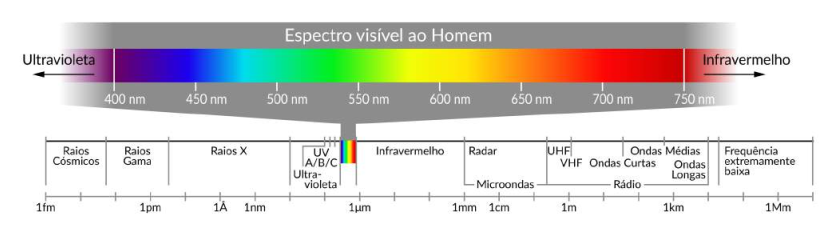
\includegraphics[width=0.985\textwidth]{./Figuras/irrad_solar.png}
    \caption{Espectro da radiação solar incluindo um detalhamento da faixa visível humana.}{Fonte: \cite{atlas2017}}
   \label{fig:irrad_solar}
\end{figure}

\newpage
\section{Sistema de produção de energia solar}

A energia solar hoje tem dois grandes usos: produção de energia térmica ou elétrica, este estudo foca na energia solar sendo usado somente para produção de eletricidade. Assim, é necessário descrever como funcionam os dispositivos envolvidos.


\subsection{Sistema de energia solar moderno}

Os sistemas de energia solar modernos, conforme mostrado na Figura \ref{fig:sistema_pv_rede}, são bem simples, estes são formados pelos painéis solares que tem como função converter a energia solar em energia elétrica em corrente contínua (CC), esta energia então é convertida para energia elétrica em corrente alternada (CA) que então pode ser utilizada para alimentar aparelhos elétricos ou fornecer energia para a rede elétrica comercial.

\begin{figure}[H]
    \centering
    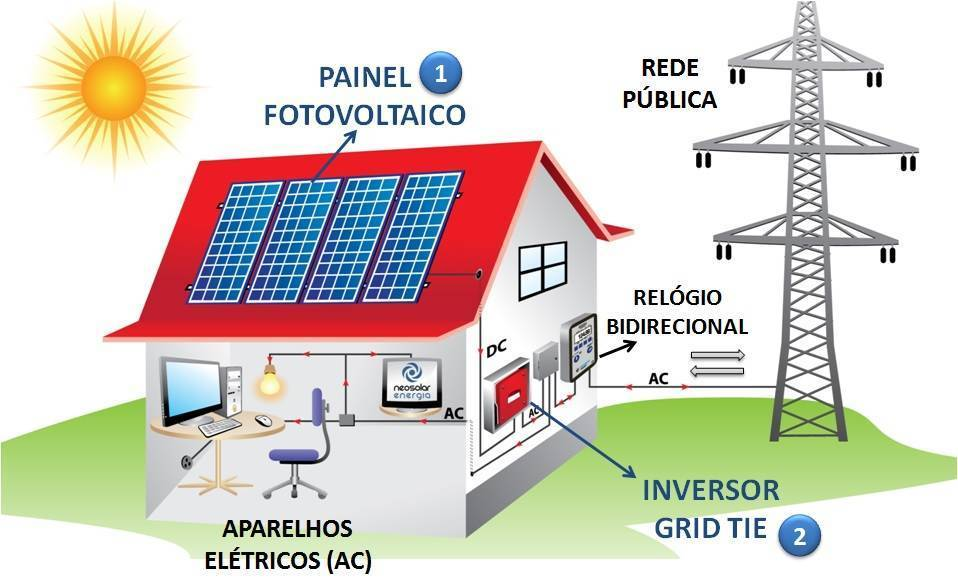
\includegraphics[width=0.85\textwidth]{./Figuras/sistema_pv_rede.jpg}
    \caption{Painel residencial solar conectado à rede.}{Fonte: \cite{neosolar}}
   \label{fig:sistema_pv_rede}
\end{figure}

A escolha de qual sistema usar depende do uso, por exemplo em um sistema no qual não há conexão com a rede elétrica, conforme se pode observar na Figura \ref{fig:sistema_pv_rede_off}, para que se possa utilizar a energia em períodos que não se tem produção é necessário implementar um sistema que seja capaz de produzir durante o dia mais energia do que é consumido e armazenar a energia extra em baterias para poder usá-la fora do horário de produção.

Para uma melhor eficiência neste sistema deve-se usar apenas otimizador de potência CC nos painéis e usar um aparelho capaz de usar diretamente a energia CC para carregar um banco de baterias. Existem inversores modernos que são capazes de, ao mesmo tempo, usar a energia CC para a conversão CC-CA e para carregar as baterias, obtendo assim a melhor eficiência do sistema.

\begin{figure}[H]
    \centering
    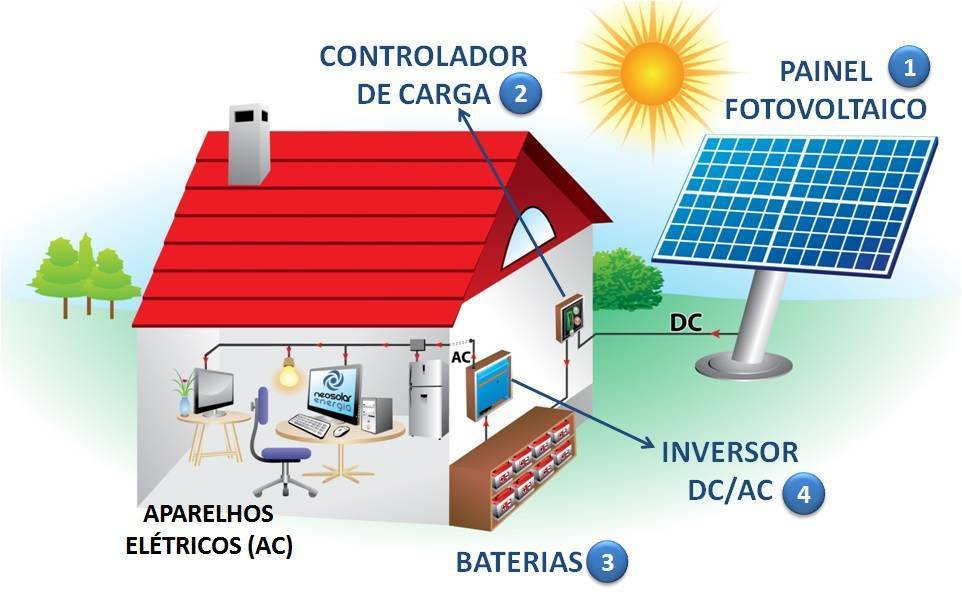
\includegraphics[width=0.85\textwidth]{./Figuras/sistema_pv_rede_off.jpg}
    \caption{Painel residencial solar off-grid.}{Fonte: \cite{neosolar}}
   \label{fig:sistema_pv_rede_off}
\end{figure}

\subsection{Dispositivos fotovoltaicos (PV)}

O dispositivo fotovoltaico, mostrado na Figura \ref{fig:BYD270P6C}, é, basicamente, um dispositivo capaz de converter energia da luz, proveniente do sol, em eletricidade através de um processo elétrico que ocorre naturalmente devido às características físicas do material do painel.

\begin{figure}[H]
    \centering
    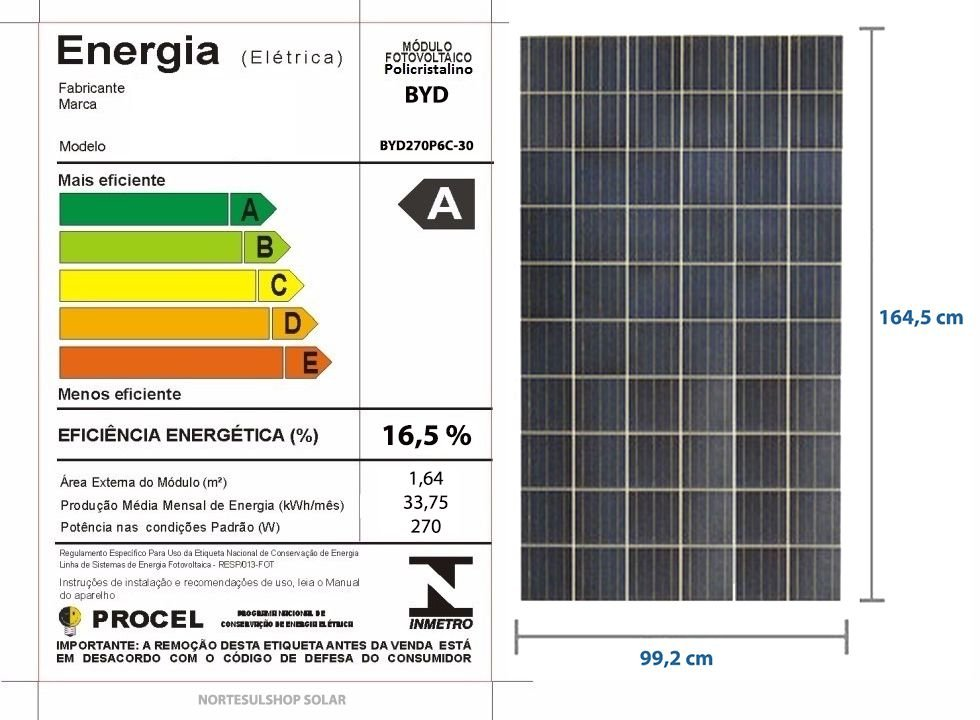
\includegraphics[width=0.9\textwidth]{./Figuras/BYD270P6C.jpg}
    \caption{Painel fotovoltaico moderno modelo BYD270P6C-30.}{Fonte: \cite{nortesulshop}}
   \label{fig:BYD270P6C}
\end{figure}

O efeito fotovoltaico (PV) foi observado já em 1839 por Alexandre Edmund Becquerel e foi objeto de investigação científica ao longo do início do século XX. Em 1954, a Bell Labs nos EUA apresentou o primeiro dispositivo solar fotovoltaico, conforme mostrado na Figura \ref{fig:1954_solar2}, que produzia uma quantidade utilizável de eletricidade e, em 1958, as células solares estavam sendo usadas em uma variedade de aplicações científicas e comerciais de pequena escala \cite{belllabs_photovoltaics}.

\begin{figure}[H]
    \centering
    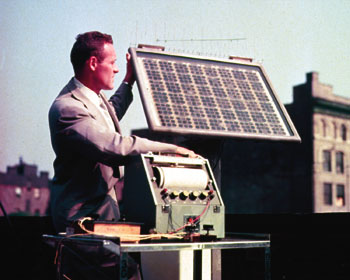
\includegraphics[width=0.8\textwidth]{./Figuras/1954_solar2.jpg}
    \caption{Engenheiro da Bell Labs testando bateria solar em 1954.}{Fonte: \cite{belllabs_photovoltaics}}
   \label{fig:1954_solar2}
\end{figure}

\begin{figure}[H]
    \centering
    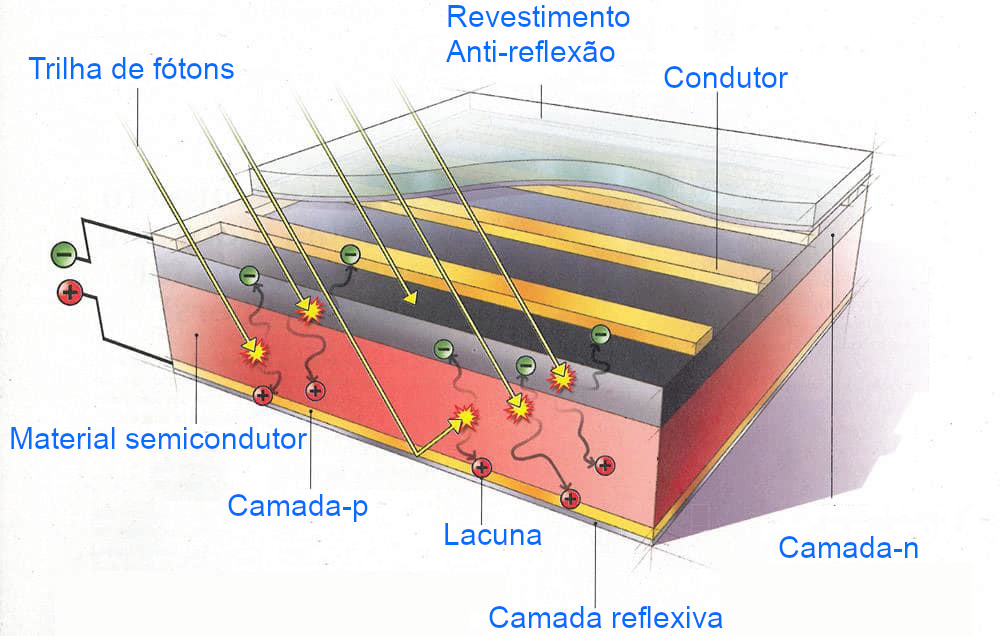
\includegraphics[width=0.8\textwidth]{./Figuras/pv-cell.jpg}
    \caption{Diagrama de uma típica célula solar de silício cristalino. Para fazer esse tipo de célula, wafers de silício de alta pureza são “dopados” com várias impurezas e fundidos. A estrutura resultante cria um caminho para a corrente elétrica dentro e entre as células solares.}{Fonte: \cite{seia}}
   \label{fig:pv-cell}
\end{figure}

A célula PV é composta de um material semicondutor. Existem vários materiais semicondutores diferentes usados em células PV, tais como, silício, filme fino, perovskite (é um mineral de óxido de cálcio e titânio composto de titanato de cálcio (CaTiO3)), orgânica, quantum dots (pontos quânticos). Porém 80-95\% dos painéis comercializados hoje em dia são feitos de silício-cristalino \cite{nrel_role}, assim o foco deste trabalho é nos painéis mais comercializados.

A luz é composta de fótons que incide na célula. A energia do fóton é transferida para um átomo do material semicondutor, especificamente elétrons, fazendo com que os elétrons saltem para um estado de maior energia, ou seja, saltem para a banda de condução. Isso deixa para trás uma lacuna na banda de valência. Este movimento do elétron resulta da energia adicionada pela luz e cria o par elétron/lacuna. Esses elétrons e lacunas agora estão livres para se mover através do material. Devido ao campo elétrico que existe como resultado da junção p-n, elétrons e lacunas se movem em direções opostas. É esse processo que cria uma corrente elétrica na célula, conforme se pode observar na Figura \ref{fig:pv-cell}. As células solares não são 100\% eficientes, em parte porque apenas certa luz dentro do espectro pode ser absorvida. Parcela da luz, que faz parte do espectro, é refletida, parte é fraca demais para criar eletricidade (infravermelho) e parte (ultravioleta) cria energia térmica em vez de eletricidade \cite{seia}.

\subsection{Eficiência e potência de painéis solares}

A eficiência do painel solar é uma medida da quantidade de luz solar (irradiação) que incide sobre a superfície de um painel solar e é convertida em eletricidade. Devido aos muitos avanços na tecnologia fotovoltaica nos últimos anos, a eficiência média de conversão do painel aumentou de 15\% para bem mais de 20\%. Este grande salto na eficiência fez com que a classificação de potência nominal de um painel de tamanho padrão (1 por 1,64 metros) mudasse de 250W para 370W \cite{cleanenergyreviews}.

A eficiência total do painel é medida em condições de teste padrão (STC), com base em uma temperatura de célula de 25° C, irradiância solar de 1000 W/m² e velocidade do vento de 1,5 m/s. A eficiência (\%) de um painel é calculada pela classificação de potência máxima (W) no STC, dividida pela área total do painel em metros (equação \ref{eq:Ef_panel}). Esta eficiência é medida com uma irradiação de 1000 W/m² sobre o painel, onde $P_{max}$ é a potência nominal máxima do painel em W e Área representa a área do painel em m²  \cite{cleanenergyreviews}.

\begin{equation}
    Efici \hat{e} ncia_{(\%)} = \frac{P_{max}}{\acute{A}rea \times 1000 \frac{W}{m^2}}
    \label{eq:Ef_panel}
\end{equation}

A eficiência geral do painel pode ser influenciada por muitos fatores, incluindo: temperatura, nível de irradiância, tipo de célula e interconexão das células. Surpreendentemente, até a cor da folha traseira protetora pode afetar a eficiência. Uma folha traseira preta pode parecer mais esteticamente agradável, mas absorve mais calor, resultando em uma temperatura de célula mais alta, o que aumenta a resistência, o que, por sua vez, reduz ligeiramente a eficiência total de conversão  \cite{cleanenergyreviews}.

Painéis solares com diferentes eficiências em relação ao seu tipo de fabricação podem ser vistos na Figura \ref{fig:pvs_pot}, painel poli Trina 250W, painéis mono 300 W e 310 W, 120 células meio corte 315 W, barramento múltiplo 335 W e na extrema direita o painel LG Neon R de alta eficiência de 20,8\% 360 W.

\begin{figure}[H]
    \centering
    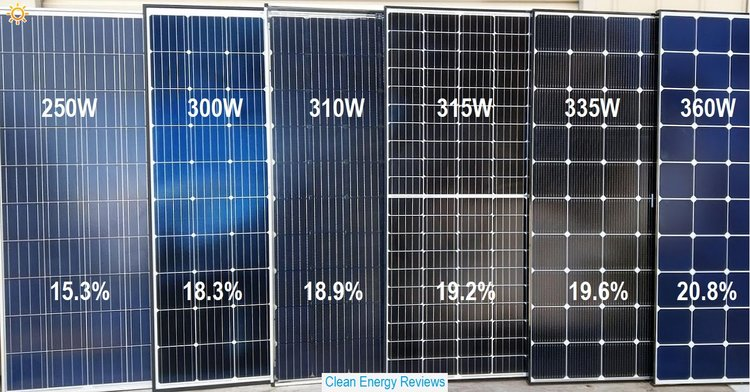
\includegraphics[width=0.8\textwidth]{./Figuras/pvs_pot.jpg}
    \caption{Eficiência e potência em relação ao tipo de painel.}{Fonte: \cite{cleanenergyreviews}}
   \label{fig:pvs_pot}
\end{figure}

O tamanho do painel e a quantidade de células individuais também são fatores que diferenciam os painéis em relação à potência máxima conforme se pode observar na Figura \ref{fig:pv_size}. Um painel de 60 células de tamanho padrão (1m x 1,7m) com eficiência de 18-20\% normalmente tem uma classificação de energia de 300-330 Watts, ao passo que um painel usando células de maior eficiência, do mesmo tamanho, pode produzir até 380W. Os painéis mais eficientes utilizam células padrão IBC tipo N de alto desempenho podem atingir até 22,6\% de eficiência e gerar 380 a 400 Watts de potência em um painel de tamanho padrão (1m x 1,7m), o modelo deste é LG MAXEON 3® \cite{Maxeon}, devido à qualidade os painéis da LG podem custar até o dobro do que um painel convencional de eficiência menor (16 a 17\%).

\begin{figure}[H]
    \centering
    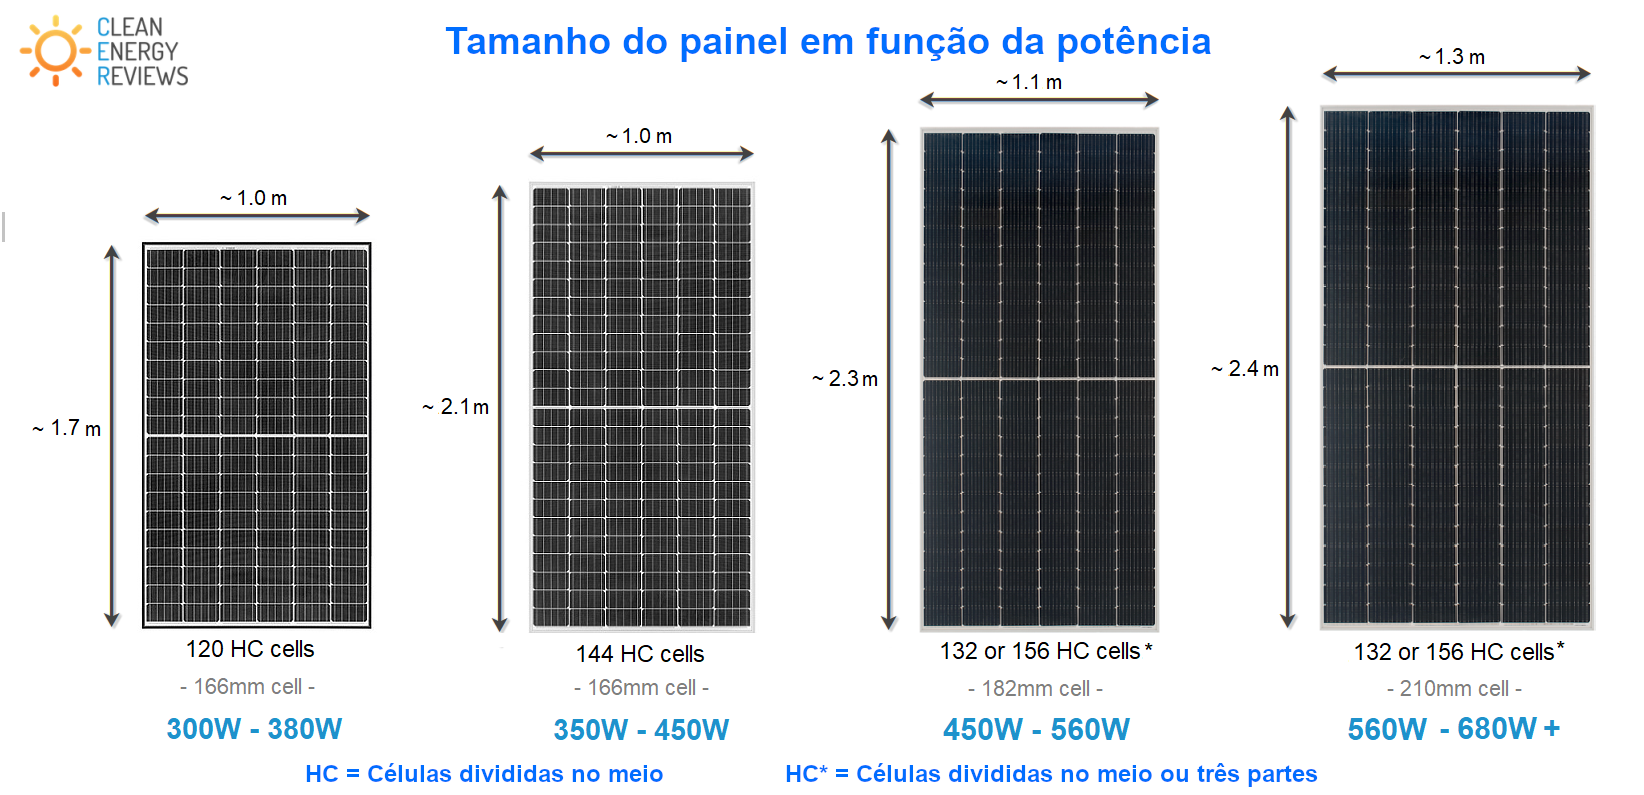
\includegraphics[width=0.975\textwidth]{./Figuras/pv_size.png}
    \caption{Tamanho do painel em função a potência.}{Fonte: \cite{cleanenergyreviews}}
   \label{fig:pv_size}
\end{figure}

\subsection{Desempenho de operação de painéis solares} \label{perf_op_pv}

Os valores nominais de eficiência e potência, discutidos na seção anterior, descrevem o desempenho do painel quando em operação ideal, mas no mundo real temos muitos fatores que influenciam essa operação. Tais como:

\begin{itemize}
  \item Irradiância solar em W/m².

  \item Temperatura do painel.
  
  \item Sombras.
  
  \item Orientação do painel.
  
  \item Localização (latitude).
  
  \item Época do ano.
  
  \item Sujeira sobre o painel.
\end{itemize}

Os dois principais fatores que que afetam o desempenho são: Irradiância solar em W/m² e Temperatura. A redução da irradiação que chega ao painel diminui a sua capacidade de produzir energia assim, todos outros fatores menos a temperatura, afetam este fator.

As curvas de desempenho, mostradas na Figura \ref{fig:pv_luz}, destacam a relação entre a irradiância e a potência do painel, assim quanto maior for a intensidade da luz que chega ao painel, maior será a potência produzida.

\begin{figure}[H]
    \centering
    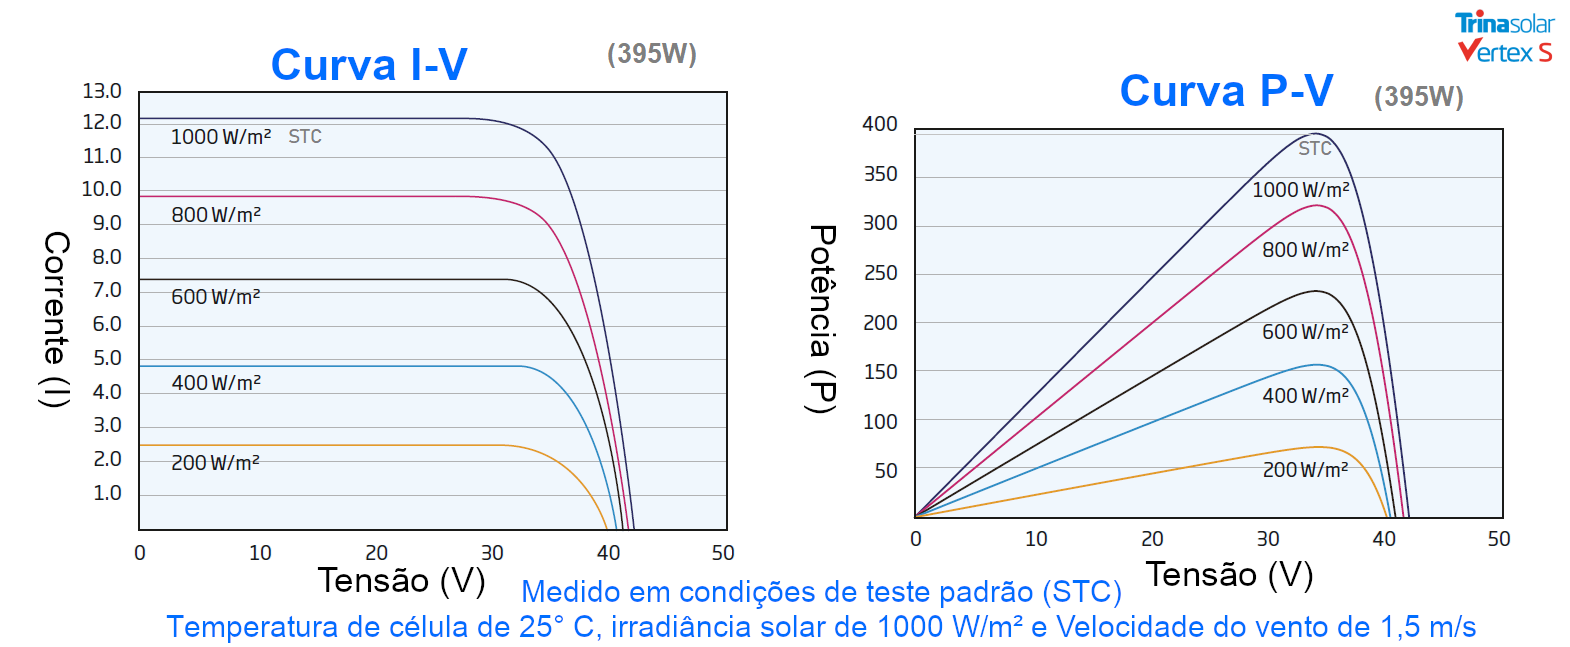
\includegraphics[width=0.95\textwidth]{./Figuras/pv_luz.png}
    \caption{Curvas de desempenho em relação à Irradiância solar.}{Fonte: \cite{cleanenergyreviews}}
   \label{fig:pv_luz}
\end{figure}

Na Figura \ref{fig:pv_temp}, é mostrado um gráfico que relaciona a potência máxima possível em relação à mudança de temperatura do painel. Esse gráfico é para o painel em questão modelo LG NeON®, que tem uma perda de potência de 0,3\% para cada 1°C de acréscimo de temperatura do painel acima dos 25°C utilizado como base para o teste ideal.

\begin{figure}[H]
    \centering
    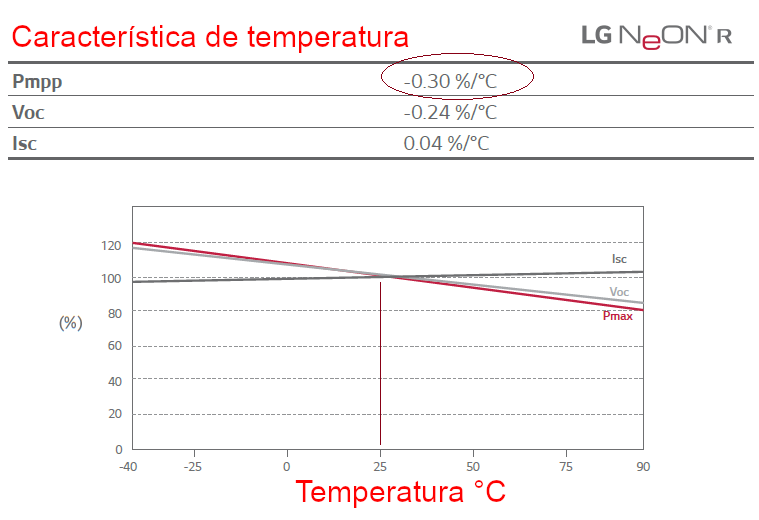
\includegraphics[width=0.85\textwidth]{./Figuras/pv_temp.png}
    \caption{Perda de potência máxima em função da temperatura.}{Fonte: \cite{LG350Q1C}}
   \label{fig:pv_temp}
\end{figure}

\subsection{Custo de painéis fotovoltaicos}

Com base em uma pesquisa de preços, realizada em abril de 2021 utilizando os sites da Tabela \ref{preco_pv}, para determinar custo de painéis, foi encontrado um preço médio que varia de R\$ 2,2 a 2,35 por Wp, ou seja um painel de 400 Wp com 19\% de eficiência, pode custar R\$ 940 e um painel de 340 Wp, com 17\% de eficiência, pode custar R\$ 760. O importante aqui é entender que um painel que tem eficiência menor pode ter seu custo menor em relação a um de maior eficiência, no entanto, se a diferença for da ordem de 6 a 7\%, o painel mais caro e mais eficiente se tornará compensador a longo prazo, pois, a quantidade de energia que este modulo pode gerar acaba compensando o custo maior em um tempo menor.

\begin{table}[htbp]
    \caption{Sites de pesquisa de preços.}
        \begin{center}
            \begin{tabular}{ >{\centering\arraybackslash} m{5cm} >{\centering\arraybackslash} m{8.5cm} }
                \hline
                Descrição & Link \\ \hline %Primeira e ultima linha adiciona \hline apos \\
                \textbf{Mercado Livre} especializado em vendas de produtos em geral & \url{https://www.mercadolivre.com.br} \\
                \textbf{Neo Solar  } especializado em produtos para energia solar & \url{https://www.neosolar.com.br} \\
                \textbf{Energia total} especializado em produtos para energia solar & \url{https://www.energiatotal.com.br} \\
                \textbf{Portal Solar} especializado em produtos para energia solar & \url{https://www.portalsolar.com.br} \\  \hline
            \end{tabular}
        \end{center}
    \label{preco_pv}
\end{table}

\section{Inversores e otimizadores de potência}

A grande maioria dos aparelhos residenciais elétricos utilizam energia CA para o seu funcionamento, no entanto, painéis solares produzem energia CC, assim, este processo de conversão pode ser realizado, basicamente, de três formas diferentes, sendo que cada uma dessas formas pode ser melhor adequada ao custo ou ao desempenho necessário de um sistema em particular.

\begin{figure}[H]
    \centering
    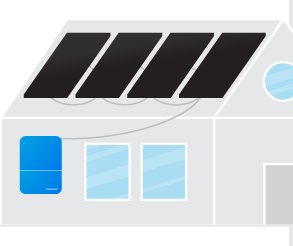
\includegraphics[width=0.48\textwidth]{./Figuras/string.png}
    \caption{Painéis conectados a um inversor.}{Fonte: \cite{EnergySage}}
   \label{fig:string}
\end{figure}

A forma mais simples é usar uma unidade central de inversão na qual os painéis são conectados em série com o inversor, conforme mostrado na Figura \ref{fig:string}. O inversor tem a função de converter a energia CC em CA de todos painéis ao mesmo tempo. Esse sistema é geralmente o mais barato mas também o menos eficiente, pois, como todos painéis estão em série, um único painel pode diminuir a potência geral do sistema em uma situação de defeito ou de sombra sobre o painel. A potência máxima dos painéis em série tem que ser menor que a potência máxima de inversão do inversor. O custo desses inversores varia de  150 a 750 R\$ por kW de potência de inversão.

\begin{figure}[H]
    \centering
    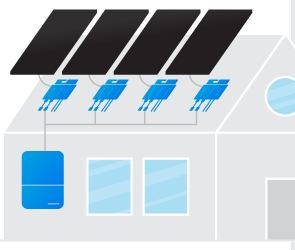
\includegraphics[width=0.48\textwidth]{./Figuras/opt.png}
    \caption{Painéis conectados a otimizador de potência e um inversor.}{Fonte: \cite{EnergySage}}
   \label{fig:opt}
\end{figure}

Uma segunda opção é utilizar um otimizador de potência individual conforme mostrado na Figura \ref{fig:string}. Esse otimizador tem a função de "condicionar" a energia CC de cada painel antes de enviá-la para o inversor, dessa forma, esse sistema consegue extrair o máximo da potência individual antes de fazer o processo de conversão CC-CA. A desvantagem desse sistema ainda está no inversor, pois a potência máxima originada nos painéis tem que ser menor que a potência máxima de inversão do inversor. O custo desse sistema é de 250 a 600 Reais por unidade. Os otimizadores são geralmente desenvolvidos especificamente para um modelo de painel ou uma série de um mesmo fabricante.

\begin{figure}[H]
    \centering
    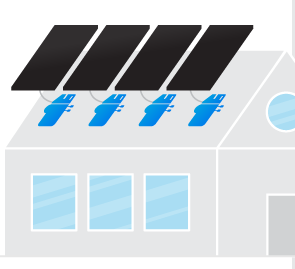
\includegraphics[width=0.48\textwidth]{./Figuras/micro.png}
    \caption{Painéis conectados a microinversores.}{Fonte: \cite{EnergySage}}
   \label{fig:micro}
\end{figure}

Um terceiro método é usar microinversores. Nessas unidades, o inversor tem a função de otimizar e converter a energia de cada painel individualmente, a Figura \ref{fig:string} ilustra esta conexão. Esses sistemas são os que vem se tornando mais populares nos últimos anos, pois é dispensada a necessidade de um inversor central, permitindo assim a expansão do sistema com mais facilidade. O custo desse sistema é de 750 a 1500 Reais por conexão de painel. Os microinversores também são geralmente desenvolvidos especificamente para um modelo de painel ou uma série de um mesmo fabricante. A maioria dos modelos de microinversores no mercado é para ser conectado a 2 ou 4 painéis ao mesmo tempo.

\section{Sistema fotovoltaico completo}

A Figura \ref{fig:edu_ci} mostra o circuito desenvolvido por \cite{tcc_edu} no seu TCC, este é um exemplo de um circuito completo desde o painel fotovoltaico até a conexão com a rede elétrica, o circuito é microcontrolado e utiliza inteligência artificial para o controle.

\begin{figure}[H]
    \centering
    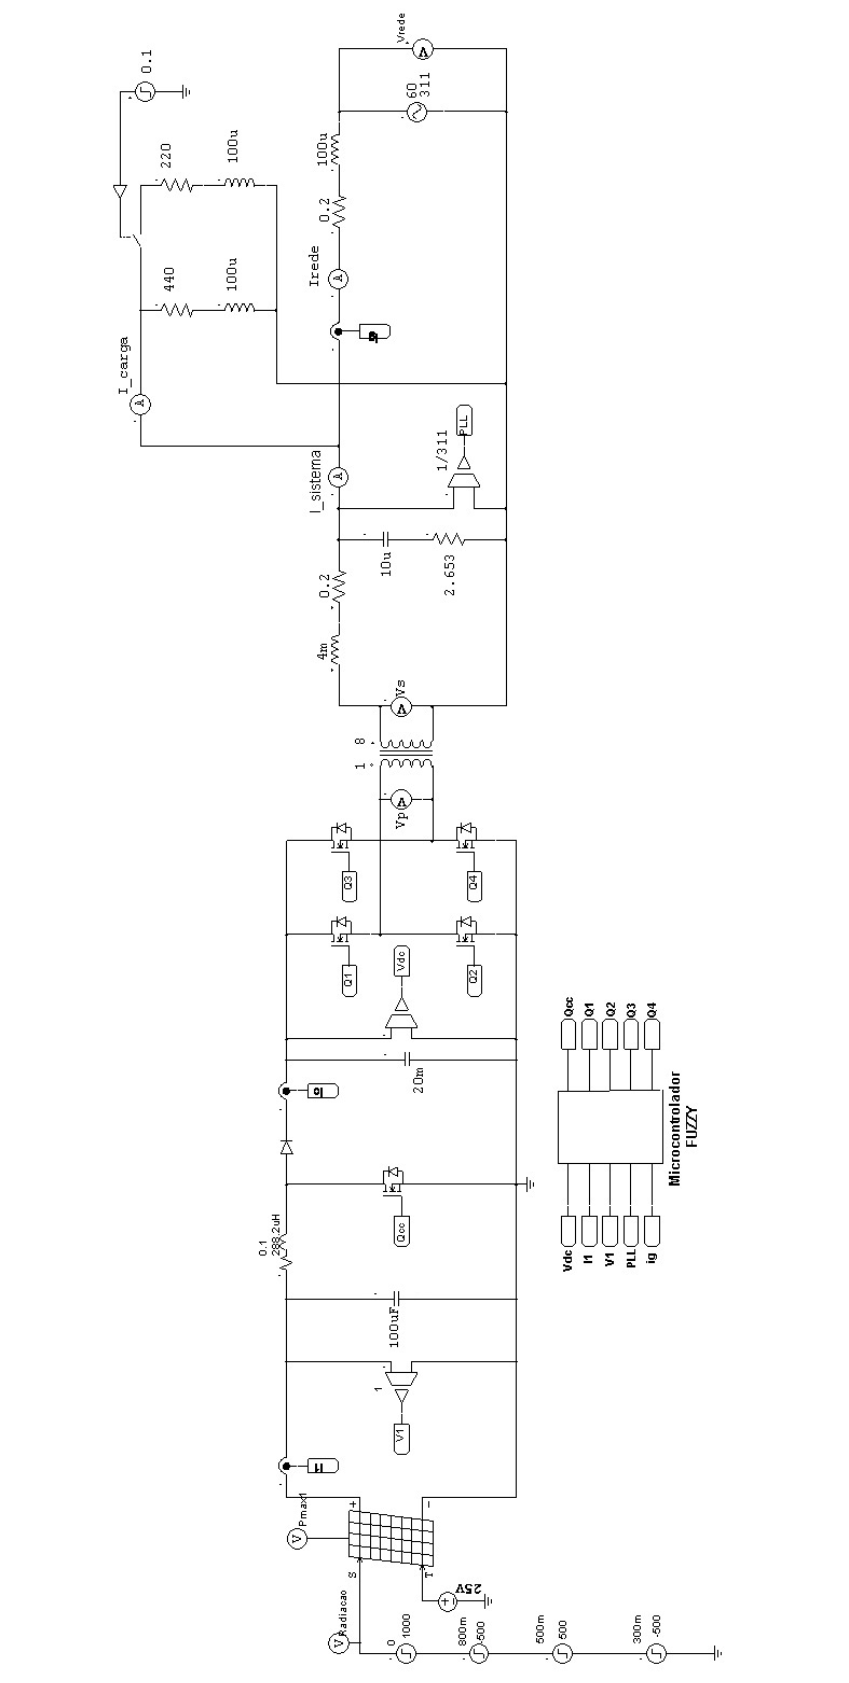
\includegraphics[width=0.7\textwidth]{./Figuras/edu_ci.png}
    \caption{Sistema fotovoltaico completo desde o painel ate a conexão com a rede.}{Fonte: \cite{tcc_edu}}
   \label{fig:edu_ci}
\end{figure}

\section{Panorama elétrico nacional}

Todos os meses, a ANEEL/ABSOLAR \cite{ABSOLAR} analisa e consolida dados do setor e produz um infográfico com o cenário da energia solar PV no País, a partir desse infográfico é possível extrair o panorama nacional elétrico, conforme descrito a seguir.

\subsection{Matriz elétrica brasileira}

\begin{figure}[H]
    \centering
    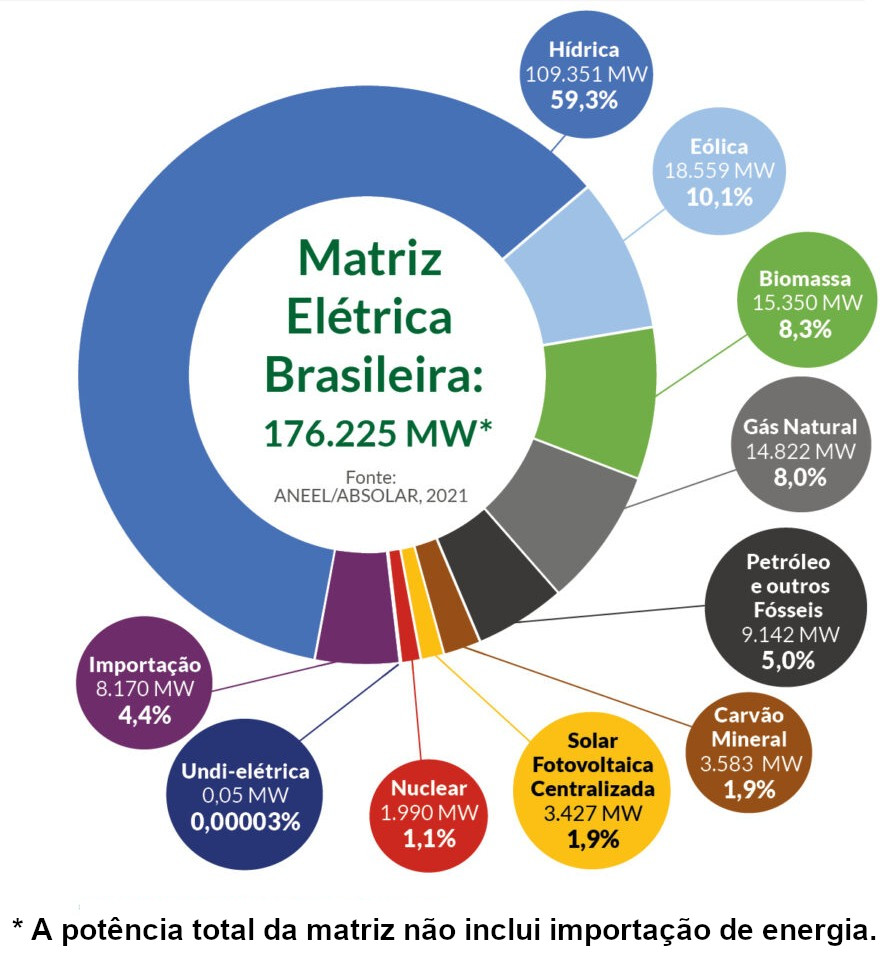
\includegraphics[width=0.75\textwidth]{./Figuras/mz_brasil.jpg}
    \caption{Matriz elétrica brasileira.}{Fonte: \cite{ABSOLAR}}
   \label{fig:mz_brasil}
\end{figure}

%Atualizar valores percentis de acordo com a atualização da imagem
Na Figura \ref{fig:mz_brasil} temos a matriz elétrica brasileira, com uma produção nacional total de 175,092 GW (esta potência total não inclui a importação de energia), sendo 59,3\% de origem hídrica, 10,1\% eólica e apenas 1,9\% solar. Essas três fontes de energia somam 71,3\% da matriz nacional e são todas de fontes de energia limpa. Os números demonstram a dependência nacional no recurso hídrico e o ainda baixo uso da energia solar em relação às outras fontes de energia.

\subsection{Evolução do uso da energia solar fotovoltaica no Brasil}

Através da distribuição da matriz elétrica nacional, é possível perceber que a dependência da energia da fonte hídrica é muito grande quando comparada às outras fontes, o que é preocupante em um cenário climático mundial incerto devido às possíveis mudanças climáticas futuras causadas pela ação humana, porém o cenário brasileiro, em relação a fontes limpas, vem mudando. Na Figura \ref{fig:ev_solar}, é possível observar a evolução da fonte solar fotovoltaica no Brasil, que tem demonstrado um crescimento exponencial nos últimos anos, comparando o potencial instalado em março de 2021 com aquele de 2012 demonstra-se um crescimento de 1210 vezes.

\begin{figure}[H]
    \centering
    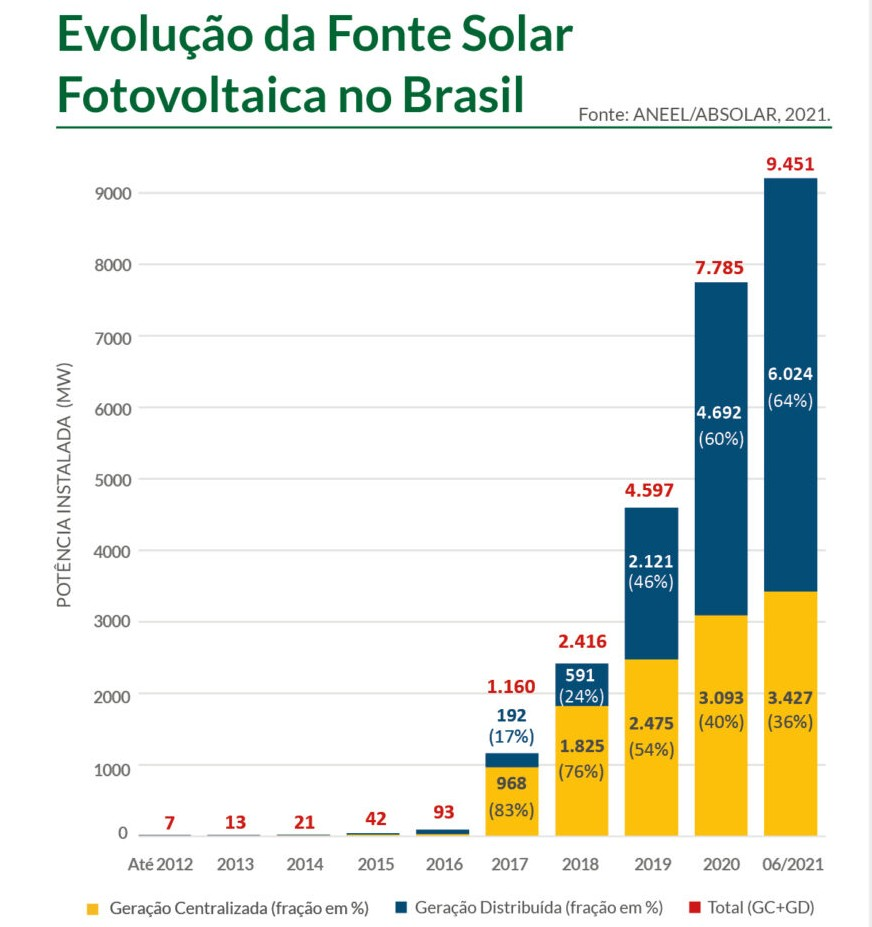
\includegraphics[width=0.9\textwidth]{./Figuras/ev_solar.jpg}
    \caption{Evolução da fonte solar fotovoltaica no Brasil.}{Fonte: \cite{ABSOLAR}}
   \label{fig:ev_solar}
\end{figure}

\subsection{Geração distribuída solar PV no Brasil}

Na Figura \ref{fig:geracao_solar_br}, se pode observar a distribuição no Brasil por classe de consumo. O perfil do potencial instalado é formado por 40,9\% residencial, 36,5\% de empresas de comércio e serviços e 13,1\% pela rural, o que demonstra uma predominância da produção solar privada.

\begin{figure}[H]
    \centering
    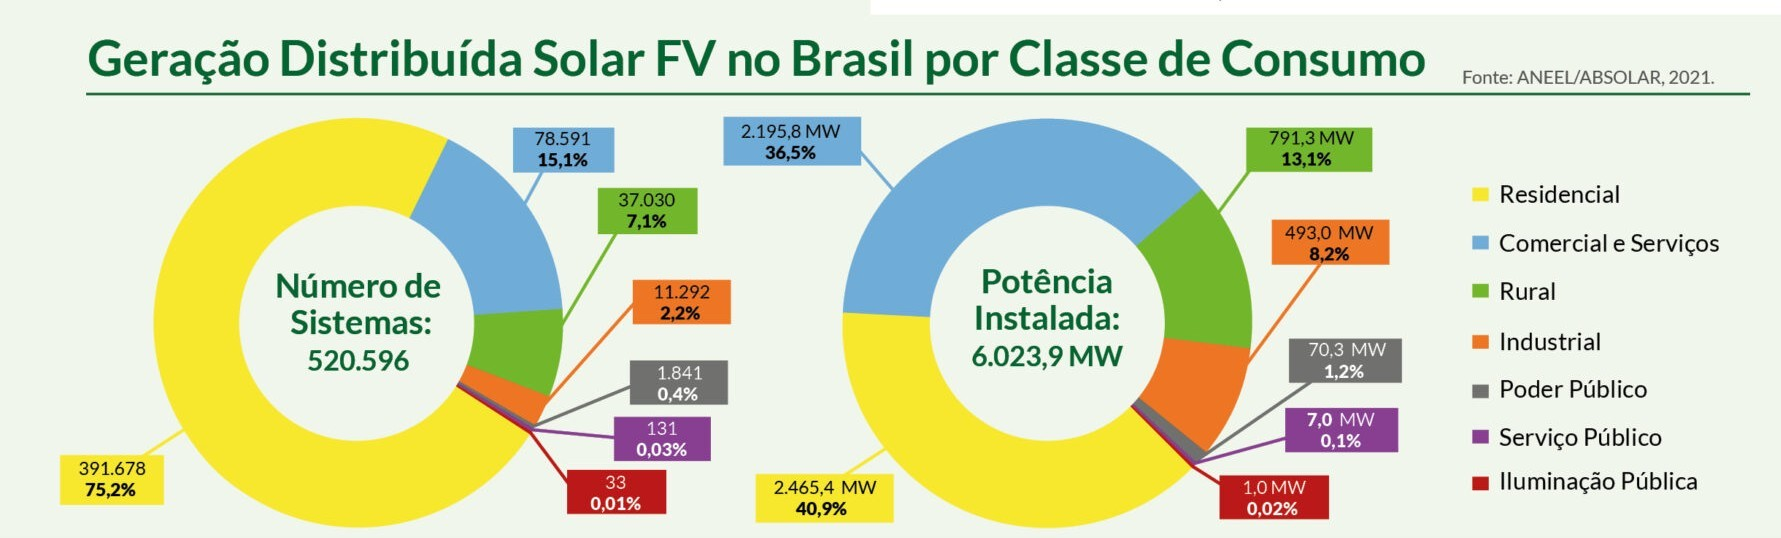
\includegraphics[width=0.985\textwidth]{./Figuras/geracao_solar_br.jpg}
    \caption{Geração distribuída solar PV no Brasil por classe de consumo.}{Fonte: \cite{ABSOLAR}}
   \label{fig:geracao_solar_br}
\end{figure}

Na Figura \ref{fig:solar_estados}, é possível observar a distribuição da geração entre os estados, sendo a liderança ocupada pelo pelo estado de Minas Gerais, seguido pelos estados do Rio Grande do Sul, São Paulo e Mato Grosso. Somente estes quatro estados são responsáveis pela produção de 50,5\% da energia solar nacional, o que demonstra uma centralização da produção e possibilidade de crescimento nacional muito grande.

\begin{figure}[H]
    \centering
    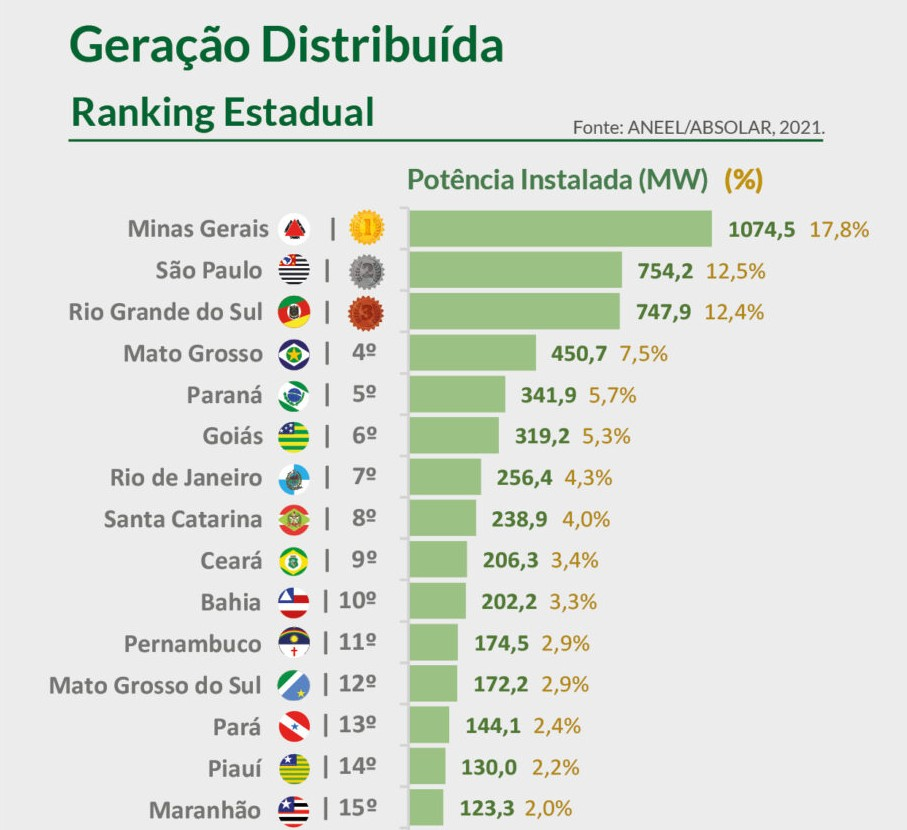
\includegraphics[width=0.75\textwidth]{./Figuras/solar_estados.jpg}
    \caption{Geração distribuída ranking estadual.}{Fonte: \cite{ABSOLAR}}
   \label{fig:solar_estados}
\end{figure}

\subsection{Potencial solar brasileiro}

A geração fotovoltaica de energia elétrica tem um grande potencial no Brasil, como indica o mapa da Figura \ref{fig:pot_geracao_solar}. No local menos ensolarado do Brasil, é possível gerar mais eletricidade solar do que no local mais ensolarado da Alemanha, por exemplo. O mapa mostra o rendimento energético anual máximo (medido em kWh de energia elétrica gerada por ano para cada kWp de potência fotovoltaica instalada) em todo o território nacional, tanto para usinas de grande porte centralizadas e instaladas em solo, como para a geração fotovoltaica distribuída integrada em telhados e coberturas de edificações. A taxa de desempenho médio anual de 80\% foi adotada para simplificar a análise e representa o desempenho de um gerador solar fotovoltaico bem projetado e instalado com equipamentos de boa qualidade e etiquetados pelo INMETRO. A concentração populacional é também mostrada através dos círculos azuis espalhados pelo território brasileiro nesta figura \cite{atlas2017}. 

\begin{figure}[H]
    \centering
    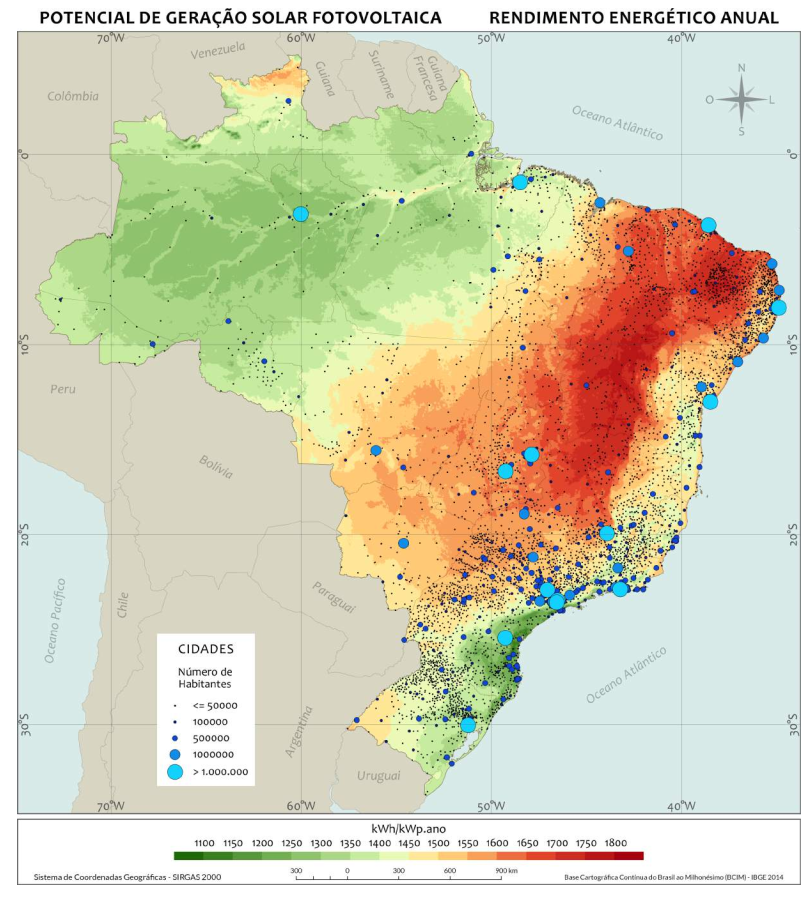
\includegraphics[width=0.85\textwidth]{./Figuras/pot_geracao_solar.png}
    \caption{Mapa do potencial de geração solar fotovoltaica em termos do rendimento energético anual para todo o Brasil (medido em kWh/kWp.ano no perfil de cores), admitindo uma taxa de desempenho de 80\% para geradores fotovoltaicos fixos e distribuição da população brasileira nas cidades.}{Fonte: \cite{atlas2017}}
   \label{fig:pot_geracao_solar}
\end{figure}

\section{Custo da energia elétrica no Brasil}

O custo da energia elétrica, como tudo no Brasil, tem uma grande carga tributária. Na Figura \ref{fig:valor_tarifa} é mostrado como é calculada a tarifa pela \cite{ANEEL_TARIFA} a fim de determinar o valor final da energia elétrica.

\begin{figure}[H]
    \centering
    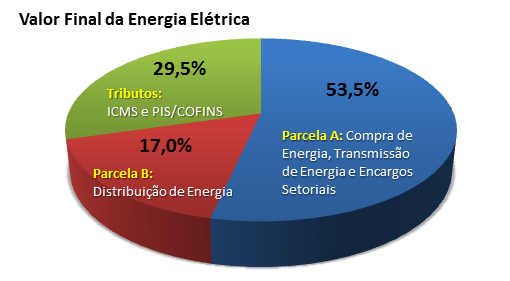
\includegraphics[width=0.9\textwidth]{./Figuras/valor_tarifa.png}
    \caption{Valor final da energia elétrica.}{Fonte: \cite{ANEEL_TARIFA}}
   \label{fig:valor_tarifa}
\end{figure}

O cálculo desta tarifa visa assegurar aos prestadores dos serviços receita suficiente para cobrir custos operacionais eficientes e remunerar investimentos necessários para expandir a capacidade e garantir o atendimento com qualidade. Os custos e investimentos repassados às tarifas são calculados pelo órgão regulador, e podem ser maiores ou menores do que os custos praticados pelas empresas \cite{ANEEL_TARIFA}.

Assim o valor final das tributações cobrado ao consumidor final é geralmente maior, usando os valores cobrados pela CEEE no estado do Rio Grande do sul, segundo a CEEE \cite{CEEE_TARIFA} o custo por kWh cobrado é de R\$ 0,54897 (Classe cliente Residencial Convencional), porém ao analisarmos uma conta de uma residência convencional veremos que o valor final pago pelo kWh é de R\$ 0,828571, o que demonstra um acréscimo de 50,8 \% em relação ao valor original, o que é uma diferença de 21,31\% em relação ao valor base da tarifa segundo a ANEEL, dentro deste valor estão incluídas perdas, encargos setoriais além dos tributos, neste custo cobrado pelo kWh pela CEEE não está incluída a bandeira tarifária.

Desde o ano de 2015, as contas de energia passaram a trazer uma novidade: o Sistema de Bandeiras Tarifárias, que apresenta as seguintes modalidades: verde, amarela e vermelha - as mesmas cores dos semáforos - e indicam se haverá ou não acréscimo no valor da energia a ser repassada ao consumidor final, em função das condições de geração de eletricidade. Cada modalidade apresenta as seguintes características \cite{ANEEL_BANDEIRAS}:

\begin{itemize}

    \item Bandeira verde: condições favoráveis de geração de energia. A tarifa não sofre nenhum acréscimo;

    \item Bandeira amarela: condições de geração menos favoráveis. A tarifa sofre acréscimo de R\$ 0,01343 para cada kWh consumidos;

    \item Bandeira vermelha - Patamar 1: condições mais custosas de geração. A tarifa sofre acréscimo de R\$ 0,04169 para cada kWh consumido.

    \item Bandeira vermelha - Patamar 2: condições ainda mais custosas de geração. A tarifa sofre acréscimo de R\$ 0,06243 para cada kWh consumido.

\end{itemize}

Sobre estes valores também incide todos acréscimos anteriores, assim o custo por kWh real cobrado pela CEEE é descrito na Tabela \ref{kwh_ceee}. Podemos ver que o custo pode chegar a ser R\$ 0,9227 o kWh, um valor 68,08 \% maior que o valor base do kWh (R\$ 0,54897) usado pela distribuidora.

\begin{table}[htbp]
    \caption{Custo final kWh cobrado pela CEEE.}
        \begin{center}
            \begin{tabular}{ >{\centering\arraybackslash} m{3cm} >{\centering\arraybackslash} m{10cm}  }
                \hline
                Bandeira & Custo kWh \newline (já com todos tributos acrescidos de 50,8\%) \\ \hline
                Verde & R\$ 0,82857\\
                Amarela & R\$ 0,84882 \\
                Vermelha 1 & R\$ 0,89143\\
                Vermelha 2 & R\$ 0,92270 \\ \hline
            \end{tabular}
        \end{center}
    \label{kwh_ceee}
\end{table}

\newpage
\section{Determinando o potencial energético de uma região}

Nas seções anteriores foi desenvolvida uma explanação sobre energia solar, sobre como utilizá-la para produção de energia elétrica e o sobre os fatores que influenciam esse processo. Nesta seção, será explicada a teoria dos processos que influenciam a produção da energia elétrica a partir da radiação solar.

Para que seja possível quantificar o quanto uma região pode gerar anualmente de energia solar, primeiro é preciso compreender os diversos fatores que influenciam esse sistema na prática. Na subseção \ref{perf_op_pv} foram definidos os principais fatores que influenciam o desempenho dos painéis solares, como, irradiância solar, temperatura do painel, sombras, orientação e etc. Nesta seção, serão definidos os fatores práticos relacionando geografia, meteorologia e componentes da irradiação que são usados para determinar e ou prever os fatores da seção anterior.

\subsection{Posição relativa entre o Sol e a Terra}

A disponibilidade do recurso energético solar e sua variabilidade espacial e temporal estão intrinsecamente relacionados a conceitos astronômicos. O primeiro dos fatores a ser considerado é a posição relativa entre o Sol e a Terra. A Terra orbita o Sol a uma distância média de cerca de 150 milhões de quilômetros, completando um ciclo a cada 365,25 dias solares. Ao longo desse período, a distância varia entre $1,47 \cdot 10^8$ km e $1,52 \cdot 10^8$ km e, como resultado, o fluxo de radiação solar (irradiância solar) oscila entre 1.325 W/m² e 1.412W/m². O valor médio da irradiância solar igual a 1.366 W/ m² é definido como a constante solar \cite{nrel} \cite{atlas2017}.

A duração do dia e a quantidade de energia solar incidente em um ponto qualquer da superfície terrestre apresenta variabilidade temporal característica de dois ciclos: o ciclo anual e o ciclo diário. O ciclo anual ocorre como consequência da inclinação em 23,45 graus do eixo axial da Terra com relação ao plano orbital do planeta em torno do Sol \cite{atlas2017}.  A Figura \ref{fig:dia_luz} mostra como a duração do dia varia ao longo do ano para diferentes latitudes. Em relação a imagem alguns exemplos de cidades que se encontram nas posições 30°S Porto Alegre RS, 20°S Vila Velha ES, 10°S Aracaju SE, 0° Macapá AM, 5°N (ponto mais extremo do estado de Roraima), são mostrados.

\begin{figure}[H]
    \centering
    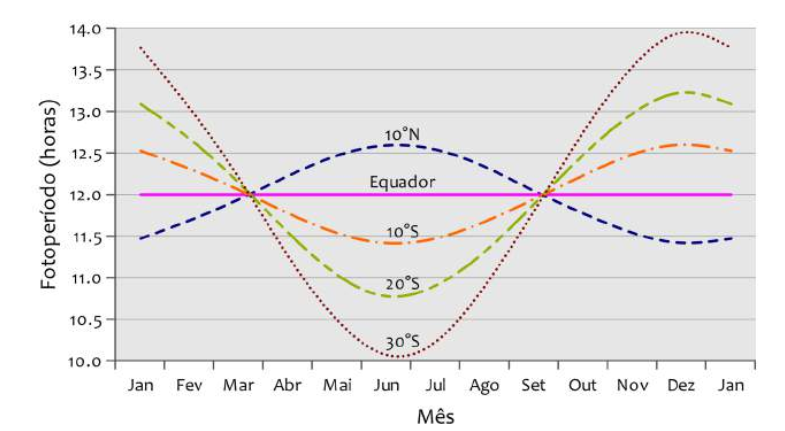
\includegraphics[width=0.9\textwidth]{./Figuras/dia_luz.png}
    \caption{Variabilidade do fotoperíodo ao longo do ano para diferentes latitudes. Deve‐se notar que o fotoperíodo apresenta maior variabilidade à medida que a localidade está mais próxima dos polos.}{Fonte: \cite{atlas2017}}
   \label{fig:dia_luz}
\end{figure}

Além do movimento de translação orbital, o movimento de rotação da Terra em torno de seu eixo está ligado ao ciclo diário da variabilidade da incidência da energia proveniente do Sol. Para descrever os dois ciclos da variabilidade da radiação solar que chega no topo da nossa atmosfera, faz‐se uso de conceitos importantes definidos geometricamente como os ângulos apresentados na Figura \ref{fig:angulo_luz}. A declinação solar ($\delta$) é o ângulo formado pela inclinação do plano equatorial da Terra e a linha de direção Sol‐Terra. Apresenta variação entre ‐23° 27’ e +23° 27’ ao longo do período de um ano. Por convenção, as declinações são consideradas negativas quando a linha de direção Sol‐Terra cruza a superfície no hemisfério Sul. A Figura \ref{fig:amplitude_luz} indica a amplitude de valores da declinação ao longo do ano \cite{atlas2017}.

\begin{figure}[H]
    \centering
    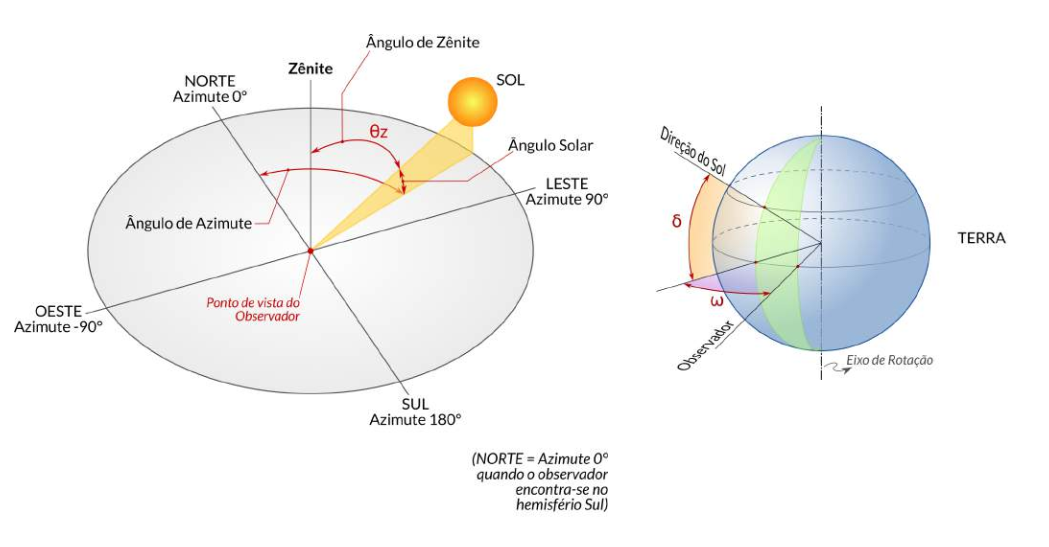
\includegraphics[width=0.7\textwidth]{./Figuras/angulo_luz.png}
    \caption{Ângulos notáveis em solarimetria. A compreensão geométrica e espacial destas variáveis permite descrever a posição do Sol em relação à um ponto na superfície terrestre e descrever numericamente a variabilidade diária e sazonal do Sol.}{Fonte: \cite{atlas2017}}
   \label{fig:angulo_luz}
\end{figure}

\begin{figure}[H]
    \centering
    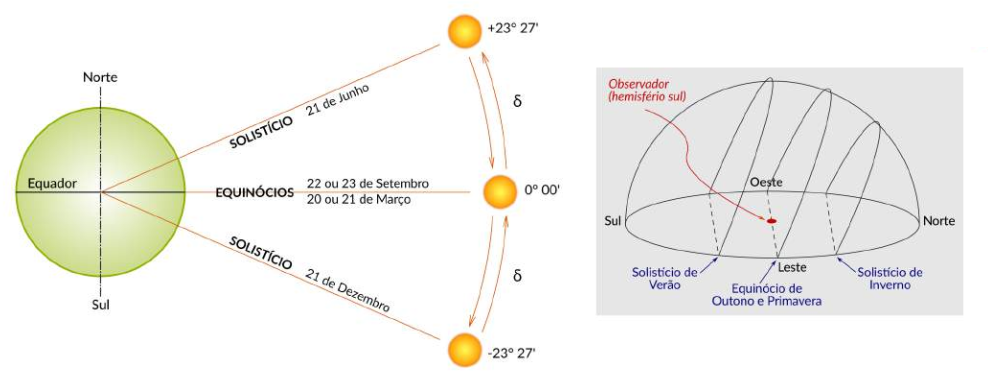
\includegraphics[width=0.7\textwidth]{./Figuras/amplitude_luz.png}
    \caption{Amplitude de valores do ângulo de declinação ao longo do ano.}{Fonte: \cite{atlas2017}}
   \label{fig:amplitude_luz}
\end{figure}

\subsection{Meteorologia para produção de energia}

A disponibilidade e a variabilidade dos recursos energéticos estão intrinsecamente associados às condições do clima da região. Isso ocorre porque sistemas meteorológicos provocam alterações na nebulosidade e nas concentrações dos gases e aerossóis, afetando os processos radiativos que atenuam a radiação solar ao longo de seu percurso na atmosfera.

O clima do Brasil é diversificado em consequência de fatores variados, como a extensão territorial, o relevo e a dinâmica das massas de ar \cite{atlas2017}.

A Figura \ref{fig:classificacao_clima} ilustra a distribuição dos climas característicos no território brasileiro segundo Köppen (Vianello e Alves, 2013). Pode‐se notar que grande parte do território brasileiro apresenta os climas tropical e subtropical (médias latitudes e altitudes elevadas no Sudeste brasileiro). Parte do sertão nordestino apresenta o clima classificado como semiárido \cite{atlas2017}.

\begin{figure}[H]
    \centering
    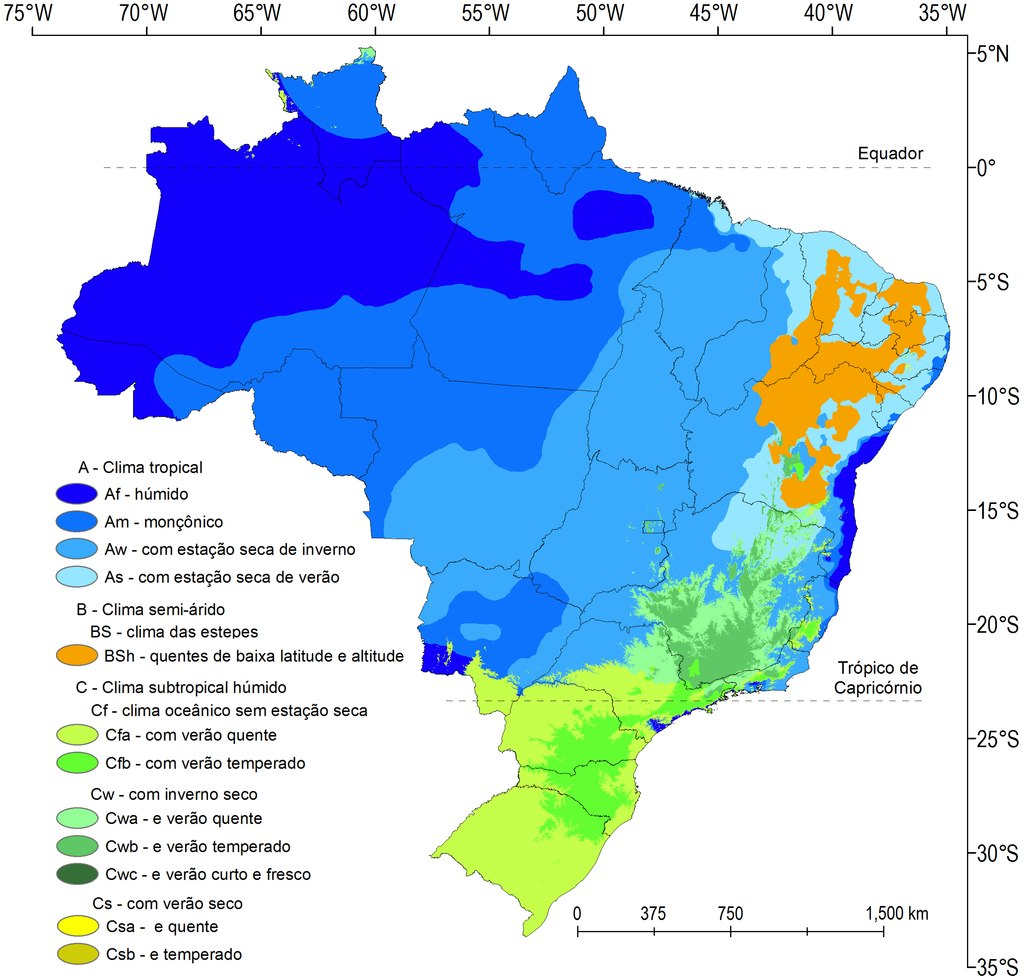
\includegraphics[width=0.85\textwidth]{./Figuras/classificacao_clima.jpg}
    \caption{Classificação climática para o Brasil segundo Köppen.}{Fonte: \cite{Koppen}}
   \label{fig:classificacao_clima}
\end{figure}

O Brasil, por possuir um território de extensões continentais abrangendo áreas de baixas e médias latitudes, experimenta diferentes padrões de precipitação em seu território, como pode ser observado na Figura \ref{fig:chuvas_clima}. O mapa representa os valores médios anuais de precipitação observados no território brasileiro determinados com base em um período de 30 anos de coleta de dados pelo Instituto Nacional de Meteorologia \cite{INMET}. No mapa, é possível identificar as características bastante distintas entre as diversas regiões do Brasil. Há regiões com precipitação média bastante elevada, como a Amazônia, e regiões com precipitação muito reduzida, como o semiárido nordestino (de duas a sete vezes menor que a observada na Amazônia) \cite{atlas2017}.

\begin{figure}[H]
    \centering
    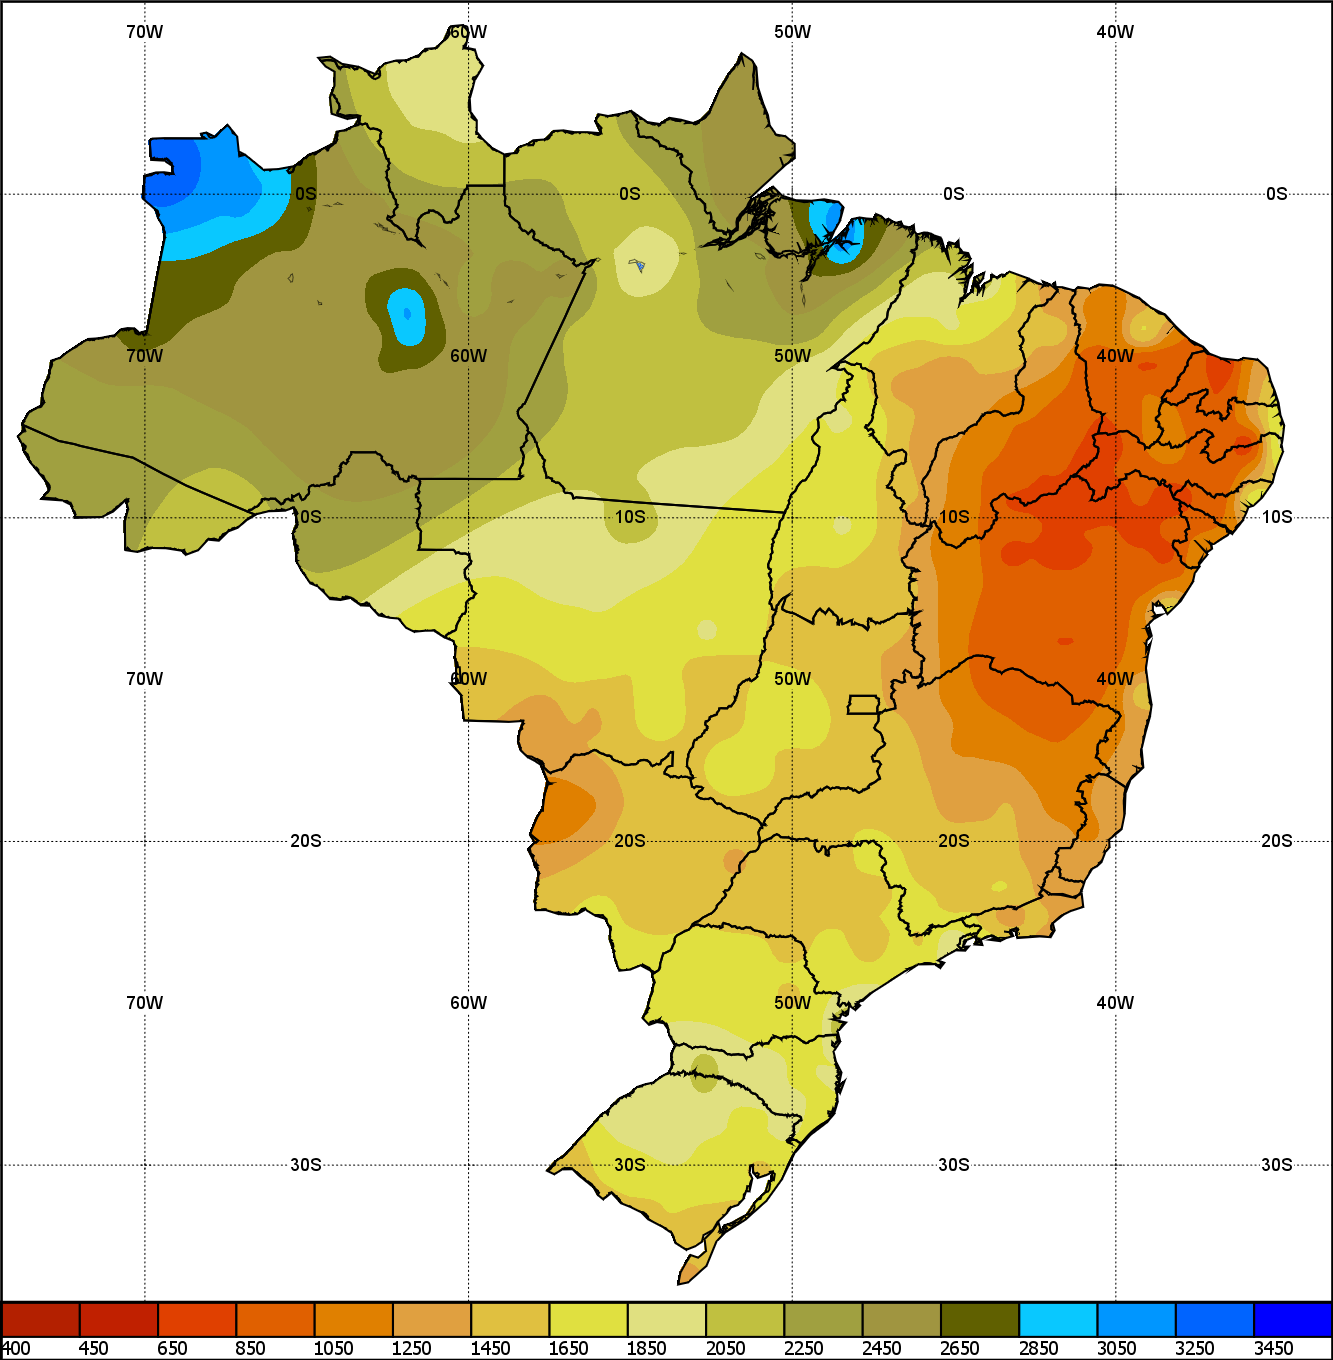
\includegraphics[width=0.8\textwidth]{./Figuras/chuvas_clima.png}
    \caption{Normal climatológica (1981‐2010)  de precipitação anual.}{Fonte: \cite{INMET}}
   \label{fig:chuvas_clima}
\end{figure}

A Figura \ref{fig:temperatura_clima} apresenta as temperaturas médias no território brasileiro. O mapa da temperatura média anual (\ref{fig:temperatura_clima}a) apresenta valores entre 14 e 30°C em grande parte do território, com maiores valores médios observados nas regiões Norte e Nordeste. As maiores médias de temperatura máxima (\ref{fig:temperatura_clima}b) são observadas em dezembro, com valores acima dos 33°C. Os valores médios anuais de temperatura mínima (\ref{fig:temperatura_clima}c) são observados em Junho na região Sul do país, chegando a 6°C nas regiões serranas. É importante mencionar que estes valores correspondem às normais climatológicas. Entretanto, extremos de temperatura fora desses intervalos são frequentemente observados no território brasileiro.

\begin{figure}[H]
    \centering
    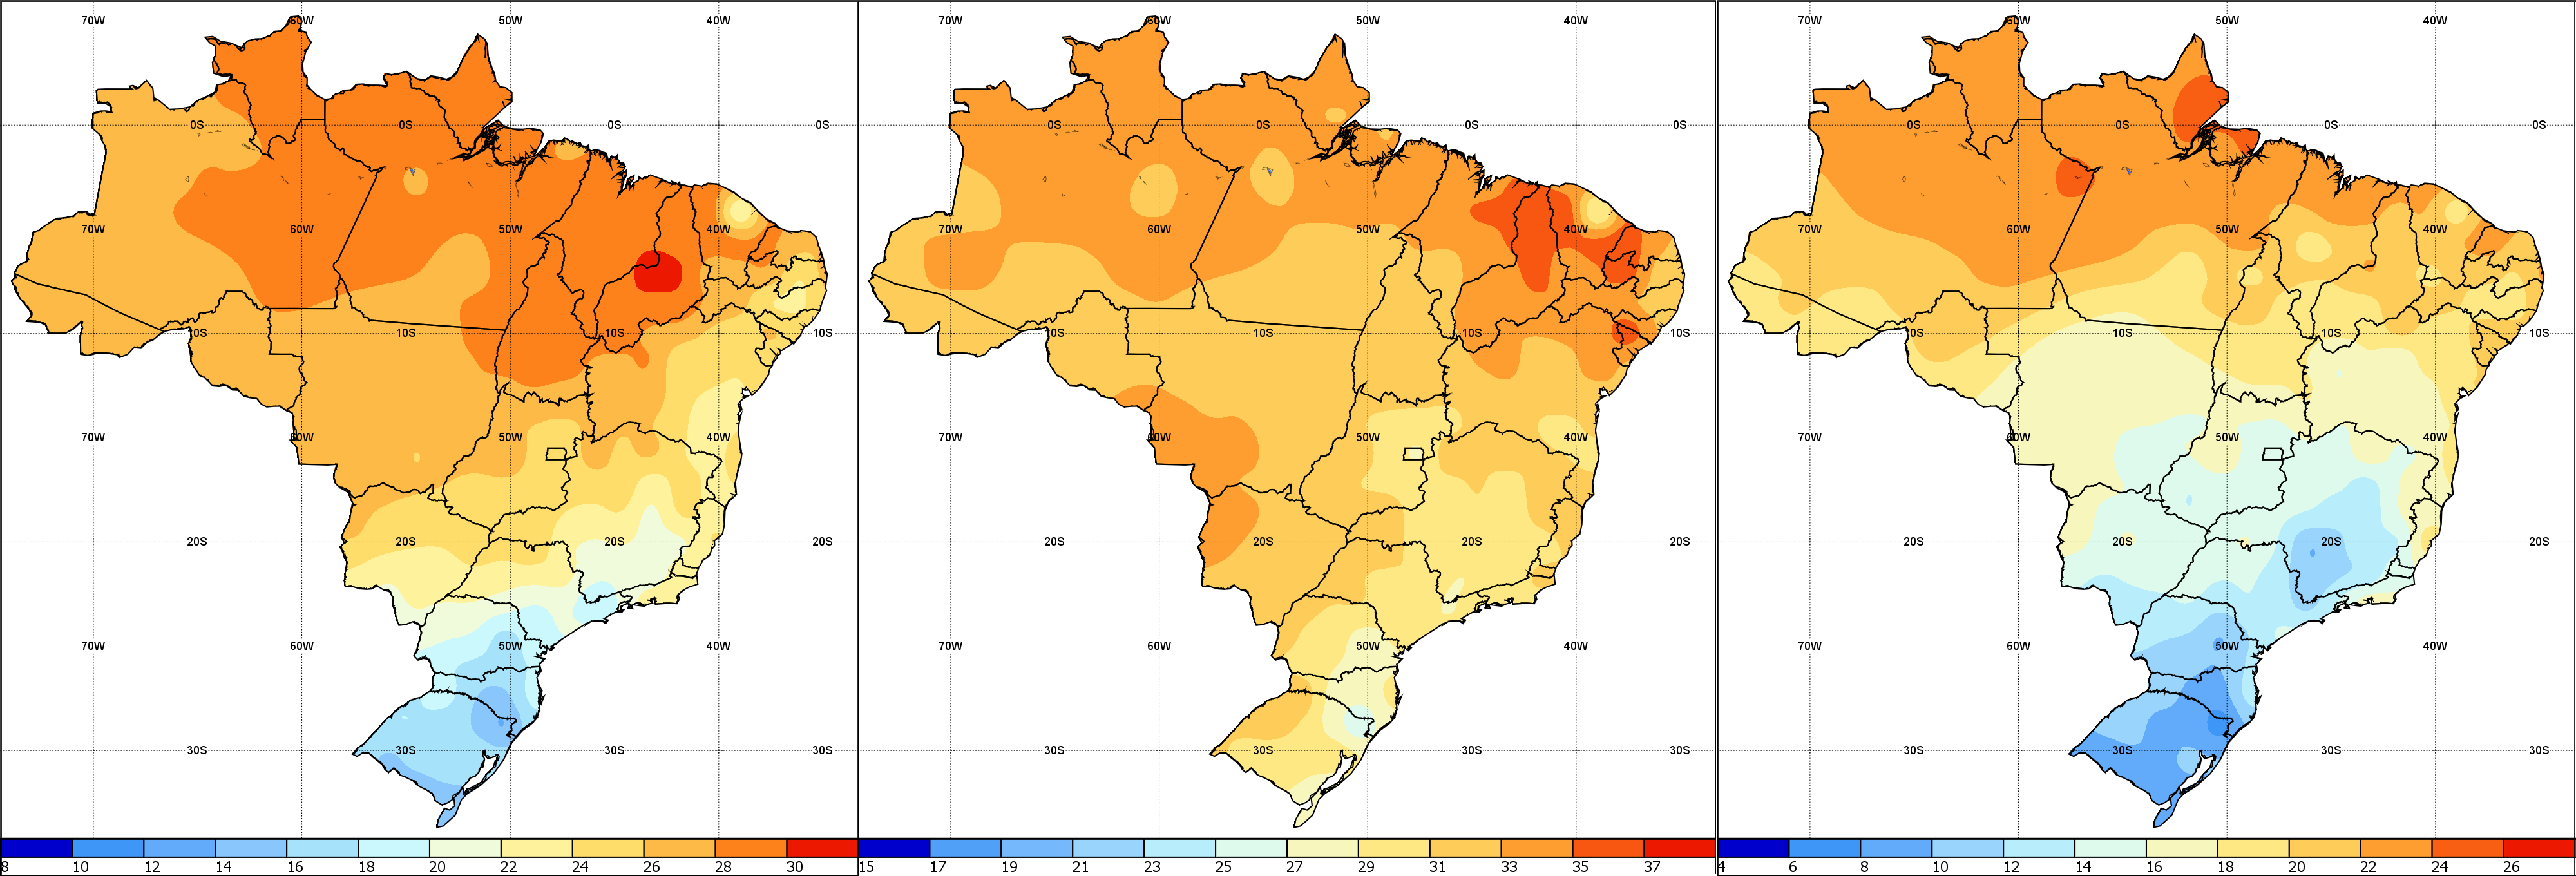
\includegraphics[width=0.95\textwidth]{./Figuras/temperatura_clima.png}
    \caption{ Normais climatológicas (1981‐2010) de temperatura no território brasileiro: (a) média anual dos valores de temperatura; (b) média de temperatura máxima observada no mês de dezembro; e (c) média de temperatura mínima observada no mês de junho.}{Fonte: \cite{INMET}}
   \label{fig:temperatura_clima}
\end{figure}

%Esta seção precisa de uma introdução e conclusão, o conteúdo é bem técnico e precisa de um bom estudo para explicar com cuidados....

%As imagens usadas aqui são originais foi buscado através da fonte que \cite{atlas2017} e não usadas as imagens do Atlas, ou seja, já foi feita uma pesquisa sobre o material do \cite{atlas2017} não é apenas uma longa citação do material original.

\section{Instrumentação e aquisição de dados}

Medidas de irradiância (W/m2) ou irradiação (Wh/m² ou J/ m²) solar “in sito” vêm sendo realizadas há algumas décadas e constituem uma base de dados muito importante para estudos de climatologia da radiação solar, para a avaliação técnica e econômica de projetos de aproveitamento do recurso energético solar e, mais recentemente, para o desenvolvimento e validação de modelos. Este tópico apresenta uma breve exposição dos principais instrumentos de medição utilizados na atualidade para aquisição de dados radiométricos com foco em atender as exigências de qualidade requeridas pelo setor energético \cite{atlas2017}.

\subsection{Piranômetro de termopilha}

O piranômetro é um instrumento destinado a medir a irradiância solar, utilizando uma termopilha que converte a energia térmica em energia elétrica. Esse instrumento pode ser visto na Figura \ref{fig:pirometro_termo}. A termopilha é revestida com uma tinta preta especial para simular a resposta de um “corpo negro” de modo que a energia radiante solar incidente é praticamente toda absorvida e convertida em calor, que, por sua vez, é convertido em uma diferença de potencial elétrico proporcional à irradiância solar incidente na termopilha. O instrumento possui sensores de temperatura do corpo e do domo para correção das medições do termopar e um ventilador (ou aquecedor), destinado a manter a temperatura do conjunto estável ao longo do dia \cite{atlas2017}.

\begin{figure}[H]
    \centering
    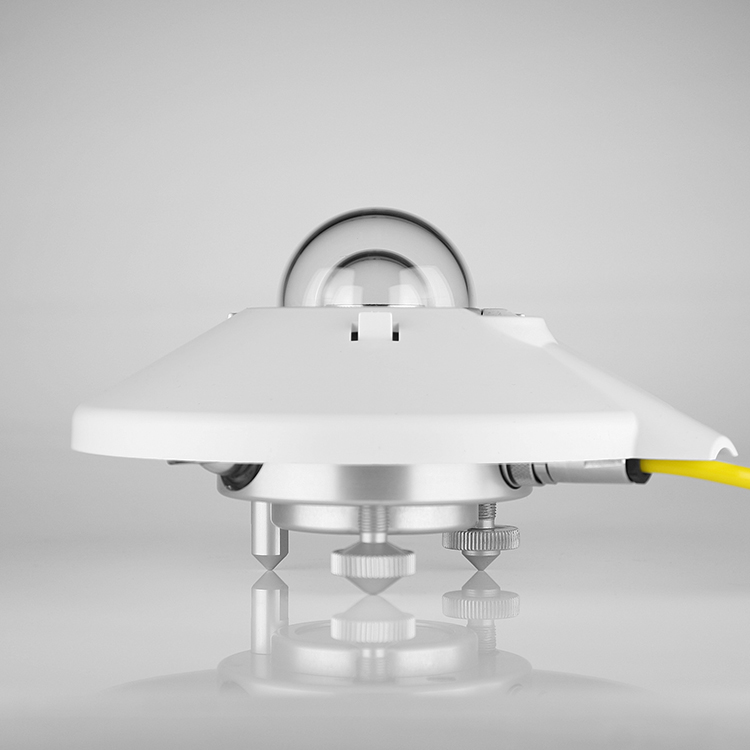
\includegraphics[width=0.5\textwidth]{./Figuras/pirometro_termo.jpg}
    \caption{ Piranômetro de fotodiodo de termopilha.}{Fonte: \cite{kippzonen}}
   \label{fig:pirometro_termo}
\end{figure}

Atualmente, o piranômetro de termopilha é o instrumento com menor incerteza para medir a radiação solar, apresentando desvios inferiores a 1\% dependendo de sua classificação \cite{atlas2017}.

\subsection{Piranômetro de fotodiodo}

O piranômetro de fotodiodo, mostrado na Figura \ref{fig:pirometro_fotodiodo}, apresenta uma célula semicondutora (fotodiodo) como elemento sensor que converte diretamente a radiação solar em corrente elétrica proporcional à irradiância solar incidente. Contudo, tais equipamentos não apresentam resposta espectral plana, conforme indicado na Figura \ref{fig:pirometro_fotodiodo_graf}. A não linearidade acarreta incertezas distintas para observações realizadas em condições de céu claro e céu totalmente nublado. Além disso, a resposta de cosseno desse equipamento é inferior, sendo também mais sensível a ruídos do que os piranômetros de termopilha, já que o princípio de funcionamento do fotodiodo é puramente elétrico e, por isso, livre de inércia térmica \cite{atlas2017}.

\begin{figure}[H]
    \centering
    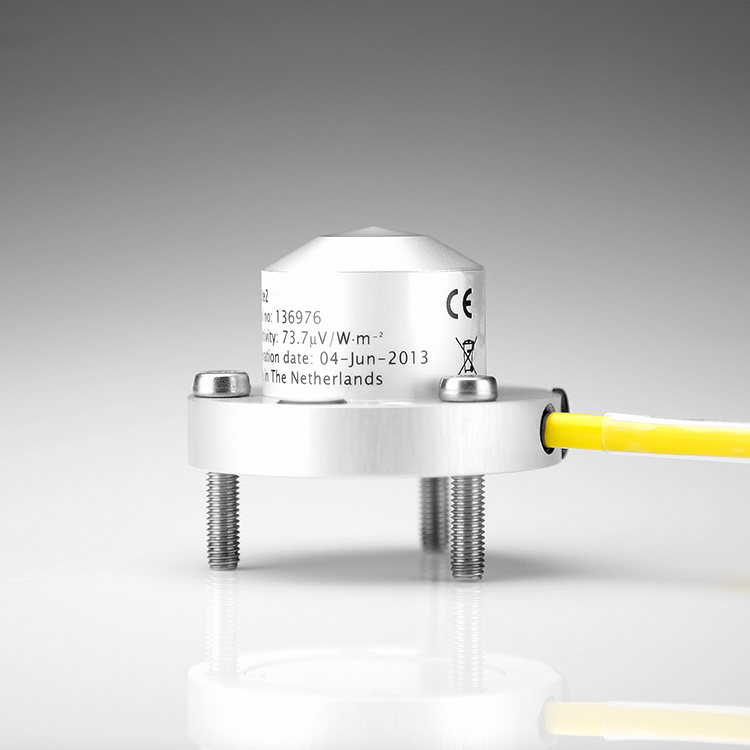
\includegraphics[width=0.5\textwidth]{./Figuras/pirometro_fotodiodo.jpg}
    \caption{ Piranômetro de fotodiodo de silício.}{Fonte: \cite{kippzonen}}
   \label{fig:pirometro_fotodiodo}
\end{figure}

\begin{figure}[H]
    \centering
    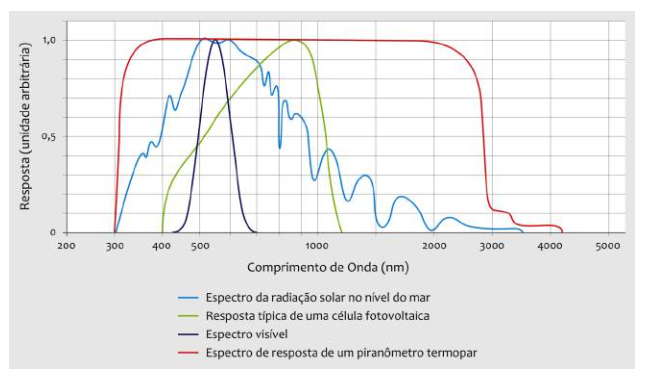
\includegraphics[width=0.95\textwidth]{./Figuras/pirometro_fotodiodo_graf.png}
    \caption{Comparação entre as curvas de resposta do piranômetro de fotodiodo de silício (linha contínua verde) e do piranômetro de termopilha (linha vermelha).}{Fonte: \cite{kippzonen}}
   \label{fig:pirometro_fotodiodo_graf}
\end{figure}

\subsection{Pireliômetro} \label{pireliometro}

O pireliômetro é um radiômetro que emprega o mesmo princípio de medida da radiação solar utilizado no piranômetro por termopilha. No entanto, este instrumento é dotado de um colimador com abertura suficiente para possibilitar que apenas a componente direta normal da radiação solar (Gn) incida no sensor. A Figura \ref{fig:pirheliometro} apresenta uma representação gráfica e uma imagem do equipamento \cite{atlas2017}.

\begin{figure}[H]
    \centering
    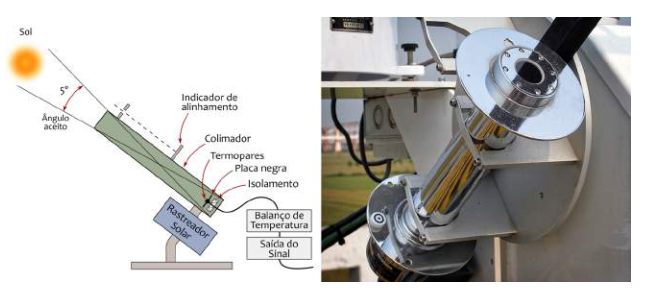
\includegraphics[width=0.95\textwidth]{./Figuras/pirheliometro.png}
    \caption{Representação gráfica e imagem de um pireliômetro.}{Fonte: \cite{kippzonen}}
   \label{fig:pirheliometro}
\end{figure}

O colimador tem um ângulo sólido de abertura de 5° por padrão internacional. O pireliômetro deve ser conectado a um sistema rastreador solar para estar sempre direcionado para o Sol. Em geral, o instrumento apresenta uma curva de resposta plana para os comprimentos de onda entre 300 a 2800 nm, cobrindo toda a faixa de ondas curtas do espectro solar. Na sua borda frontal, possui um pequeno orifício que projeta a luz solar sobre um ponto marcado na borda inferior, permitindo que o operador verifique diariamente o correto alinhamento do equipamento \cite{atlas2017}.

\subsection{Sistemas de sombreamento}

A aquisição de dados da componente difusa da radiação solar também é realizada com uso de piranômetros, com preferência para os equipados com termopilha em razão do melhor desempenho conforme descrito anteriormente. No entanto, a aquisição de dados da radiação solar difusa só pode ser realizada com a supressão da incidência do feixe de radiação solar direta sobre o sensor. Duas técnicas são comumente empregadas para sombrear o sensor termopilha do piranômetro: o anel de sombreamento e a esfera de sombreamento com rastreador solar. Ambas estão ilustradas na Figura \ref{fig:sis_sombra}.

\begin{figure}[H]
    \centering
    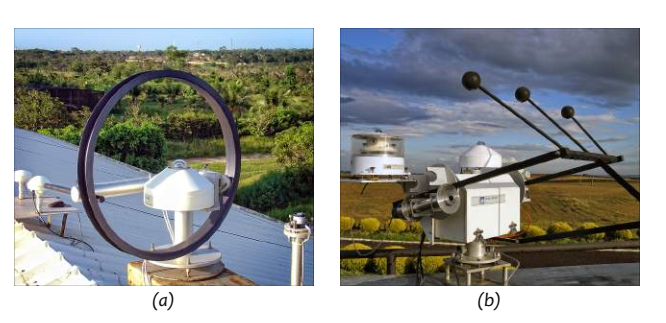
\includegraphics[width=0.9\textwidth]{./Figuras/sis_sombra.png}
    \caption{Sistemas para sombreamento do piranômetro utilizados na aquisição de dados de radiação difusa: anel de sombreamento (a) e esfera de sombreamento com rastreador solar (b).}{Fonte: \cite{atlas2017}}
   \label{fig:sis_sombra}
\end{figure}

O anel de sombreamento é um uma cinta circular ou semi‐ circular que se adapta ao suporte do piranômetro de tal forma que a sombra do anel esteja sempre projetada exatamente sobre o elemento sensor durante a trajetória aparente do Sol na abóboda celeste (eclíptica) conforme se pode visualizar na Figura \ref{fig:sis_sombra}.a. O anel deve ser ajustado periodicamente para compensar a variação sazonal da declinação solar durante o ano. Embora, relativamente barato e simples, este procedimento apresenta a desvantagem de bloquear também uma pequena porção da radiação difusa; contudo, existem equações de correção disseminadas na literatura científica para compensar tal efeito \cite{atlas2017}.

Mais preciso, contudo com maior custo, é o procedimento que faz uso do rastreador solar, também conhecido como seguidor solar mostrado na Figura \ref{fig:sis_sombra}.b. Trata‐se de um sistema robotizado que, uma vez posicionado corretamente com relação ao Sol e configurado com as coordenadas geográfica do local, passa a seguir de forma automática a trajetória do Sol. Um sistema de esferas pintadas de preto fosco, acoplado ao rastreador solar evita a incidência do feixe de radiação solar direta sobre o elemento sensor, eliminando assim o problema relacionado com o encobrimento parcial do céu causado pelo anel de sombreamento. O sistema robótico é muito preciso e, em casos de desalinhamento, conta com um detector de Sol que permite o realinhamento automático em condições de céu claro \cite{atlas2017}.

\subsection{Estações meteorológicas automáticas do INMET}

Estações meteorológicas automáticas (EMA’s) operadas pelo INMET conforme mostrado na Figura \ref{fig:estacao_meteorologicas}, são empregadas para fins de estudos meteorológicos e monitoramento ambiental. Operam de forma automática e desatendida, com dados transmitidos via satélite e estão distribuídas por todo o território nacional.

\begin{figure}[H]
    \centering
    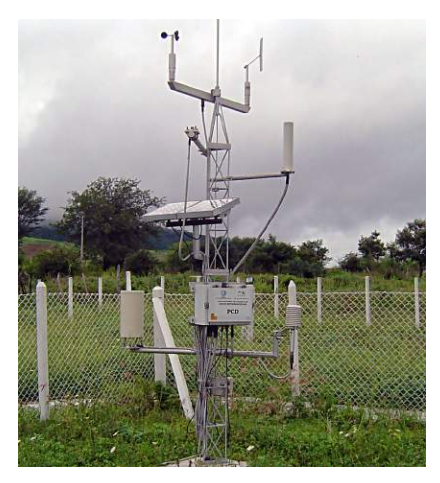
\includegraphics[width=0.8\textwidth]{./Figuras/estacao_meteorologicas.png}
    \caption{Foto de estação automática de coleta de dados.}{Fonte: \cite{atlas2017}}
   \label{fig:estacao_meteorologicas}
\end{figure}

Uma estação meteorológica automática é composta de uma unidade central de memória (datalogger) conectada aos sensores de parâmetros meteorológicos, como pressão atmosférica, temperatura e umidade relativa do ar, precipitação, radiação solar, direção e velocidade do vento. A estação integra os valores observados minuto a minuto e os disponibiliza automaticamente a cada hora.

\subsection{Estações de coleta de dados de radiação solar}

A Figura \ref{fig:estacao_solar} apresenta uma estação típica da rede SONDA. Rastreadores solares, como mostrado em primeiro plano, são utilizados para aquisição de dados da componente difusa (Gdif) e direta normal (Gn) em oito estações: os dados da componente direta são coletados através de pireliômetros. As demais estações da rede SONDA não realizam aquisição da componente direta normal e a componente difusa é coletada com uso de anel de sombreamento, que requer ajuste periódico manual de posicionamento \cite{atlas2017}.

\begin{figure}[H]
    \centering
    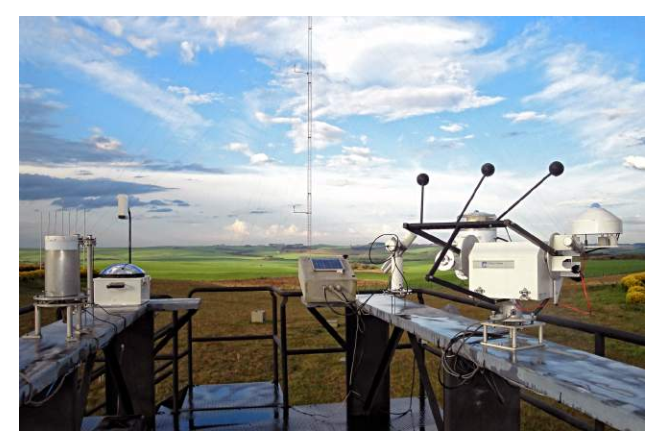
\includegraphics[width=0.8\textwidth]{./Figuras/estacao_solar.png}
    \caption{Foto de uma estação de coleta de dados de radiação solar da rede SONDA, localizada em São Martinho da Serra, RS, empregada na validação do Atlas.}{Fonte: \cite{atlas2017}}
   \label{fig:estacao_solar}
\end{figure}

As estações da rede SONDA também estão equipadas para aquisição de dados de radiação de onda longa, com o emprego de pirgeômetros, de radiação fotossinteticamente ativa (PAR) e de iluminância, além de variáveis meteorológicas tipicamente observadas em estações meteorológicas automáticas: velocidade e direção do vento, umidade relativa do ar, temperatura do ar, precipitação e pressão atmosférica. A medição da atenuação por aerossóis atmosféricos é realizada com uso de fotômetros solares instalados em cinco das estações. Todas essas observações são utilizadas em conjunto para análise e verificação da consistência dos dados medidos \cite{atlas2017}.

A rede de EMA’s operada pelo INMET compreende cerca de 900 estações meteorológicas típicas distribuídas pelo território nacional e integradas ao sistema de observação global da WMO. Trata‐se da rede de coleta de dados de maior abrangência no território brasileiro. Os pontos azuis da Figura \ref{fig:etacoes_inmet} ilustram a localização dessas EMA’s e os vermelhos as estações SONDA \cite{atlas2017}.

\begin{figure}[H]
    \centering
    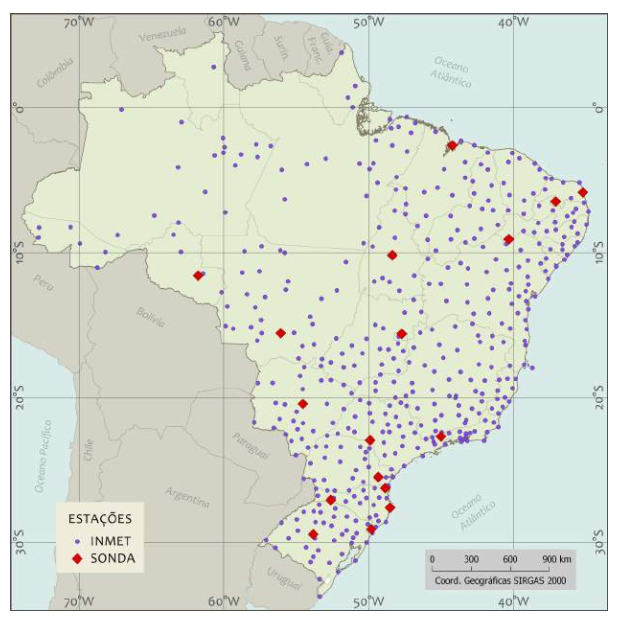
\includegraphics[width=0.95\textwidth]{./Figuras/etacoes_inmet.png}
    \caption{Localização das estações da rede SONDA e das EMA 's da rede de observação meteorológica operada pelo INMET utilizadas na validação do Atlas.}{Fonte: \cite{atlas2017}}
   \label{fig:etacoes_inmet}
\end{figure}

\section{Modelagem de sistemas de energia fotovoltaica}\label{modelo_sadia}

Para o desenvolvimento deste projeto escolheu-se utilizar um modelo matemático para determinar a desempenho de um sistema PV. O laboratório nacional (EUA) Sandia desenvolveu uma biblioteca de livre acesso que permite modelar todos os processos de um sistema PV. A Figura \ref{fig:sandia_model} ilustra o processo. Nos seguintes subtópicos será descrito todo o processo e as equações utilizadas no modelo deste trabalho.

\begin{figure}[H]
    \centering
    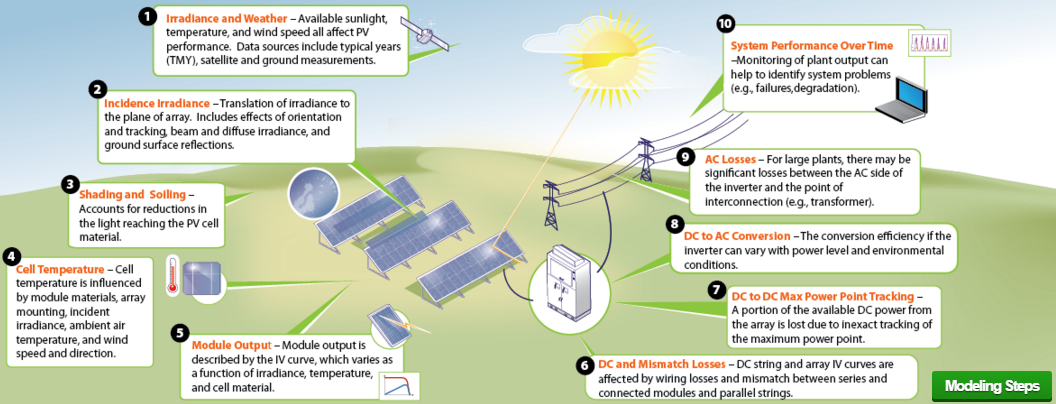
\includegraphics[width=0.975\textwidth]{./Figuras/sandia_model.png}
    \caption{Modelo PV PMC do Sandia.}{Fonte: \cite{sandia}}
   \label{fig:sandia_model}
\end{figure}

\subsection{Sobre o Sandia}

Sandia é um laboratório multiprograma de engenharia e ciência operado pela National Technology and Engineering Solutions de Sandia, LLC. Que opera para a Administração Nacional de Segurança Nuclear do Departamento de Energia dos EUA (NNSA). O Sandia está facilitando um grupo colaborativo de profissionais fotovoltaicos (PV Performance Modeling Collaborative ou PVPMC). Este grupo está interessado em melhorar a precisão e o rigor técnico dos modelos e análises de desempenho fotovoltaico. Tais modelos são usados para avaliar o desempenho (índice de desempenho) e determinar o valor futuro dos projetos de geração PV (expresso como o rendimento de energia previsto) e, por extensão, influenciar como os projetos e tecnologias PV são percebidos pela comunidade financeira em termos de investimento e risco. Uma maior confiança na precisão dos modelos de desempenho levará a menores custos de financiamento e a um aumento no número de projetos que são construídos. O PVPMC oferece um espaço colaborativo para trabalhar em prol desses objetivos \cite{sandia}.

\subsection{Plano da matriz (POA)}

Nesta etapa, os dados de irradiância são transpostos para o plano da matriz. Os submodelos incluídos nesta etapa incluem vários algoritmos de rastreamento de posição, estimativas para a refletividade do solo (albedo) e modelos para calcular a irradiância difusa na matriz do céu \cite{sandia}.

O cálculo da irradiância incidente na matriz é fundamental para modelar o desempenho de um sistema fotovoltaico. Este cálculo envolve:

\begin{itemize}
  \item Definir ou determinar a orientação da matriz, que pode ser fixa ou variável no tempo (matrizes de rastreamento).

  \item Estimar as contribuições dos componentes do feixe e da irradiância difusa (céu difuso e difuso refletido no solo).
\end{itemize}

Alternativamente, pode-se medir o plano de irradiância da matriz diretamente com um piranômetro, célula de referência ou módulo de referência montado na mesma orientação da matriz. O analista deve compreender as diferentes características desses sensores para garantir que quaisquer correções subsequentes feitas na irradiância do POA medida sejam apropriadas \cite{sandia}.

Uma etapa fundamental no cálculo do desempenho do PV é determinar a irradiância incidente no plano da matriz (POA) em função do tempo. Esta irradiância POA é dependente de vários fatores, incluindo:

\begin{itemize}
  \item Posição do Sol.
  
  \item Orientação dos painéis (fixa ou com rastreamento).
  
  \item Componentes de irradiação (diretos e difusos).
  
  \item Refletividade da superfície do solo (Albedo).
  
  \item Sombreamento (obstruções próximas e distantes).
\end{itemize}

A matematicamente a irradiância POA $E_{POA}$ é:

\begin{equation}
    E_{POA} = E_b + E_g + E_d
    \label{eq:poa}
\end{equation}

Onde $E_b$ é a componente do feixe, $E_g$ é a componente de reflexão do solo e $E_d$ é a componente de difusão. Todas essas grandezas são detalhadas a seguir.

\newpage
\subsection{Componente de irradiância do feixe POA $E_b$}

A componente de irradiância do feixe plano de matriz (POA) é calculada ajustando a irradiância normal direta (DNI) pelo ângulo de incidência (AOI) da seguinte maneira:

\begin{equation}
    E_{b} = DNI \times cos(AOI)
    \label{eq:eb}
\end{equation}

\subsection{Irradiância normal direta (DNI)}

A irradiância normal direta (DNI) pode ser medida diretamente por meio de um radiômetro de cavidade absoluta. Os radiômetros de cavidade absoluta são considerados o método mais preciso de medição da radiação solar e formam a base da Referência Radiométrica Mundial (WRR). No entanto, os radiômetros de cavidade absoluta não são projetados para uso externo contínuo e autônomo \cite{sandia}.

Assim, o principal método de medição de DNI é com um instrumento chamado pireliômetro.

\subsection{Ângulo de incidência (AOI)}

O ângulo de incidência (AOI) entre os raios do Sol e o arranjo fotovoltaico pode ser determinado como:

\begin{equation}
    AOI = cos^{-1}[cos(\theta_Z)cos(\theta_T) + sin(\theta_Z)sin(\theta_Z)cos(\theta_A - \theta_{A,Matriz})]
    \label{eq:aoi}
\end{equation}

Onde $\theta_A$ e $\theta_Z$ são os ângulos solares de azimute e zênite, respectivamente e $\theta_T$ e $\theta_{A,Matriz}$ são os ângulos de inclinação e azimute da matriz, respectivamente.

A convenção do ângulo de azimute é definida como graus a leste do norte (por exemplo, Norte = 0, Leste = 90, Oeste = 270). O azimute da matriz é definido como o vetor normal horizontal da superfície da matriz. Uma matriz voltada para o sul tem um azimute de matriz de 180 graus. A inclinação da matriz é definida como o ângulo da horizontal. A Figura \ref{fig:sun_position} ilustra esses ângulos.

\begin{figure}[H]
    \centering
    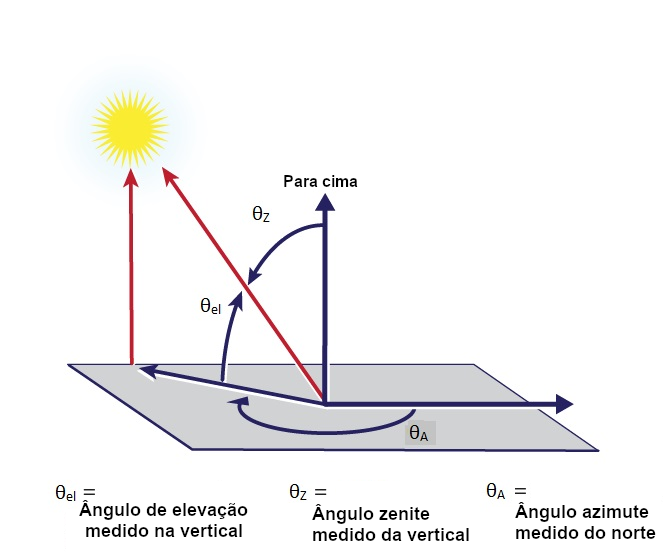
\includegraphics[width=0.6\textwidth]{./Figuras/sun_position.png}
    \caption{Definição dos ângulos azimute e zênite.}{Fonte: \cite{sandia}}
   \label{fig:sun_position}
\end{figure}

\subsection{A irradiância em uma superfície inclinada que é refletida do solo $E_g$}

A irradiância em uma superfície inclinada que é refletida do solo $E_g$, é calculada como uma função da irradiância no solo $GHI$, do albedo que é a fração da irradiação horizontal global refletida, e do ângulo de inclinação da superfície do painel $\theta_{T, superf\acute{i}cie}$:

\begin{equation}
    E_g = GHI \times albedo \times \frac{1 - cos(\theta_{T, superf\acute{i}cie})}{2}
    \label{eq:eg}
\end{equation}

\begin{figure}[H]
    \centering
    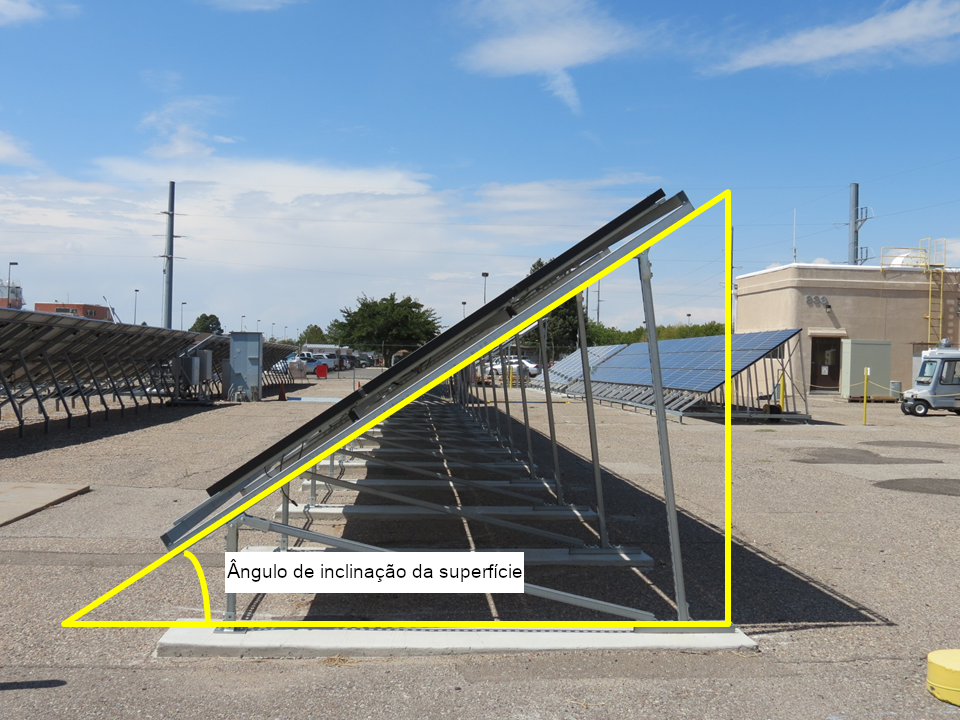
\includegraphics[width=0.6\textwidth]{./Figuras/angulo_superficie.png}
    \caption{Ângulo de inclinação da superfície do painel.}{Fonte: \cite{sandia}}
   \label{fig:angulo_superficie}
\end{figure}

\subsection{Irradiância horizontal global GHI}

A irradiância horizontal global (GHI) é a quantidade de irradiância terrestre que cai em uma superfície horizontal à superfície da terra. GHI pode ser medido com uma variedade de instrumentos. O instrumento mais comumente usado para medir GHI é chamado de piranômetro, que possui um ângulo de visão hemisférico (180°). A marca registrada de um piranômetro é uma resposta verdadeira do cosseno ao ângulo incidente, ou seja, a resposta do piranômetro a um feixe de luz é proporcional ao cosseno do ângulo incidente do feixe. A maioria dos piranômetros utiliza um sensor de termopilha para detectar a luz que entra; no entanto, piranômetros como o Licor LI-200 usam um dispositivo fotovoltaico com um difusor. Os piranômetros baseados em termopilha têm uma resposta espectral plana à luz de entrada, enquanto os piranômetros baseados em materiais PV terão sensibilidade espectral de acordo com os materiais usados no sensor. Os piranômetros que usam um sensor PV respondem quase que instantaneamente às mudanças na irradiância, ao contrário de suas contrapartes termopilha que levam de 1 a 15 segundos para atingir uma resposta completa a uma mudança gradual na irradiância. O GHI também pode ser medido com uma célula fotovoltaica de referência, que terá sensibilidade espectral e geralmente não exibirá uma resposta real ao cosseno \cite{sandia}.

Se o GHI não puder ser medido diretamente, ele pode ser calculado a partir da irradiância normal direta (DNI) e da irradiância horizontal difusa (DHI) usando a seguinte equação:

\begin{equation}
    GHI = DHI + DNI \cdot cos(\theta_Z)
    \label{eq:ghi}
\end{equation}

\subsection{Irradiância horizontal difusa  DHI}

A irradiância horizontal difusa (DHI) é a irradiância terrestre recebida por uma superfície horizontal que foi espalhada ou difundida pela atmosfera. É o componente da irradiância horizontal global que não vem do feixe do sol (onde “feixe” é um campo de visão de 5° concêntrico ao redor do sol). Muito parecido com a irradiância horizontal global, o DHI é normalmente medido com um piranômetro; entretanto, neste caso, a luz direta do sol é bloqueada a fim de remover o componente do feixe da radiação. O sol pode ser bloqueado por uma bola ou disco que remove apenas o cone de 5° em torno do sol e deve utilizar um rastreador para sombrear continuamente apenas o sensor do piranômetro. O piranômetro também pode ser sombreado por uma faixa de sombreamento horizontal ou vertical (o primeiro não requer rastreador, o último requer um rastreador horizontal); no entanto, as faixas de sombra geralmente são menos precisas, pois removem parte da luz difusa. Esta luz difusa deve ser medida e corrigida por um fator de correção dependente da localização e do tempo.

Se a irradiância horizontal difusa não for medida diretamente, ela pode ser calculada de maneira semelhante à irradiância horizontal global por (\ref{eq:ghi}).

\subsection{Albedo}

Albedo é a fração da irradiação horizontal global refletida. Quando a superfície é muito escura $Albedo \approx 0$ e quando a superfície é branca brilhante ou metálica $Albedo \approx 1$.

O software de modelagem PVsyst \cite{pvsyst} fornece a seguinte orientação para estimar um valor apropriado para albedo:

\begin{itemize}
  \item Ambiente urbano 0,14 - 0,22.

  \item Grama 0,15 - 0,25 / Grama fresca 0,26.

  \item Neve fresca 0,82.

  \item Neve molhada 0,55-0,75.

  \item Asfalto seco 0,09-0,15.

  \item Asfalto Úmido 0,18.

  \item Betão 0,25-0,35.

  \item Ladrilhos vermelhos 0,33.

  \item Alumínio 0,85.

  \item Cobre 0.74.

  \item Novo aço galvanizado 0,35.

  \item Aço galvanizado muito sujo 0,08.

\end{itemize}

A Figura \ref{fig:dni-dhi-ghi} ilustra as irradiações DNI, DHI, GHI e o albedo sobre um painel.

\begin{figure}[H]
    \centering
    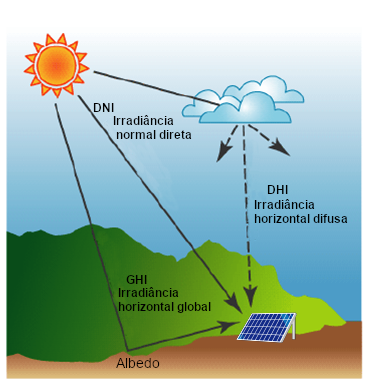
\includegraphics[width=0.5\textwidth]{./Figuras/dni-dhi-ghi.png}
    \caption{Ilustração das irradiações DNI, DHI, GHI e o albedo.}{Fonte: \cite{esri}}
   \label{fig:dni-dhi-ghi}
\end{figure}

\subsection{Irradiância difusa do céu $E_d$ }

A radiação difusa na cúpula do céu é normalmente dividida em vários componentes:

\begin{itemize}
  \item[--] O componente isotrópico, que representa a irradiância uniforme da cúpula do céu;
  
  \item[--] O componente difuso circunsolar, que representa o espalhamento direto da radiação concentrada na área imediatamente ao redor do sol;
  
  \item[--] O componente de clareamento do horizonte.
  
\end{itemize}

Os modelos publicados usam diferentes abordagens semi-empíricas para estimar a combinação desses componentes.

\subsection{Modelo isotrópico para irradiância difusa do céu}

O modelo isotrópico para radiação difusa do céu é o mais simples dos modelos POA difuso do céu e forma a base sobre a qual os modelos mais precisos são construídos. O modelo isotrópico do céu difuso assume que a radiação difusa da cúpula do céu é uniforme no céu. A irradiância difusa do céu POA ($E_{d,iso}$) é calculada como uma fração da irradiância horizontal difusa medida (DHI) como:

\begin{equation}
    E_{d,iso} = DHI \times \frac{1 + cos(\theta_{T, superf\acute{i}cie})}{2}
    \label{eq:ed_iso}
\end{equation}

\subsection{Modelo empírico para irradiância difusa do céu}

Este modelo empírico para irradiância difusa do céu foi desenvolvido no Sandia por David King e funcionou muito bem nas instalações da Sandia (melhor, na verdade, do que qualquer um dos outros modelos quando comparados). O modelo determina a irradiância difusa da superfície inclinada do céu ($E_d$) usando o ângulo de inclinação da superfície ($\theta_{T, superf\acute{i}cie}$), irradiância horizontal difusa (DHI), irradiância horizontal global (GHI) e ângulo zênite do sol ($\theta_Z$) como:

\begin{equation}
    E_{d} = DHI \times \frac{1 + cos(\theta_{T, superf\acute{i}cie})}{2} + GHI \times \frac{(0,012 \theta_Z - 0,04) \times (1 - cos(\theta_{T, superf\acute{i}cie})}{2}
    \label{eq:ed_emp}
\end{equation}

Observe que o primeiro termo é simplesmente o modelo isotrópico de difusão do céu. O segundo termo é um termo de correção empírico para explicar os efeitos de clareamento circunsolar e do horizonte. Todos os ângulos estão em graus.

\subsection{Modelo temperatura do modulo}

Sandia propõe o seguinte modelo para estimar a temperatura do módulo:

\begin{equation}
    T_m = POA \cdot (e^{a + b \cdot WS}) + T_a
    \label{eq:tm}
\end{equation}

Onde:

\begin{itemize}
  \item $POA$ Irradiância solar Incidente no modulo em W/m².

  \item $T_a$ Temperatura ambiente °C.
  
  \item $WS$ velocidade do vento m/s.
\end{itemize}

Neste caso, a e b são parâmetros que dependem da construção e dos materiais do módulo, bem como da configuração de montagem do módulo. A tabela \ref{tm_tabela} lista os valores representativos para esses parâmetros para vários tipos e configurações de módulo comuns.

\begin{table}[htbp]
    \caption{Valores dos parâmetros da construção e do material do modulo PV}
        \begin{center}
            \begin{tabular}{ >{\centering\arraybackslash} m{5cm} >{\centering\arraybackslash} m{3cm} >{\centering\arraybackslash} m{2cm} >{\centering\arraybackslash} m{2cm} >{\centering\arraybackslash} m{2cm} } 
                \hline
                Módulo & Montagem & a & b & $\Delta_T$ \\ \hline %Primeira e ultima linha adiciona \hline apos \\
                Vidro/célula/vidro & telhado aberto & -3,47 & -0,0594 & 3  \\
                Vidro/célula/vidro & telhado fechado & -2,98 & -0,0471 & 1  \\
                Vidro/célula/polímero & telhado aberto & -3,56 & -0,075 & 3  \\
                 Vidro/célula/polímero & telhado fechado & -2,81 & -0,0455 & 0  \\  \hline
            \end{tabular}
        \end{center}
    \label{tm_tabela}
\end{table}

\subsection{Modelo temperatura da célula}

O modelo de temperatura da célula Sandia estima a temperatura da célula a partir da temperatura do módulo, $T_m$, plano de irradiância da matriz $POA$, e um parâmetro de diferença de temperatura, $\Delta_T$. Este parâmetro de diferença define a diferença de temperatura entre a temperatura do módulo e da célula.

A equação do modelo é:

\begin{equation}
    T_c =  T_m + \frac{POA}{E_0} \Delta_T
    \label{eq:tc}
\end{equation}

Onde $E_0$ é uma irradiância de referência (1000 W/m²).

\subsection{Ponto de Potência máxima CC}

Esses tipos de modelos são projetados para prever um ponto (geralmente o ponto de potência máxima ($P_{pm}$) ou pontos (por exemplo,$P_{pm}$,$V_{oc}$, e $I_{sc}$) na curva IV como uma função de variáveis  (por exemplo, irradiância, temperatura da célula e conteúdo espectral, para exemplo).

O modelo proposto calcula a potência CC dos painéis a partir do valor nominal de potência do painel $P_{m0}$ à temperatura de célula calculada $T_c$ e a irradiância $POA$. Presume-se que a eficiência da matriz diminua a uma taxa linear em função do aumento da temperatura, governada pelo coeficiente de temperatura do painel $\gamma$ em $^{\circ} C^{-1}$. A temperatura de referência da célula $Tr$ é 25°C e a irradiância de referência $E_0$ é 1000 W/m² \cite{PVWatts}.
\newline

Para irradiância $POA > 125$ W/m²:

\begin{equation}
    P_{pm} = \frac{POA}{E_0} P_{m0} [1 + \gamma(T_c - T_r)]
    \label{eq:pmp}
\end{equation}

Para irradiância $POA < 125$ W/m²:

\begin{equation}
    P_{pm} = \frac{0,008 (POA)^2}{E_0} P_{m0} [1 + \gamma(T_c - T_r)]
    \label{eq:pmp2}
\end{equation}

Porém estas equações não são perfeitas, pois apresentam um erro demonstrado na Figura \ref{fig:PVWatts_erro}, assim \cite{Marion} no instituto NREL apresentou com detalhes deste erro e uma solução.

\begin{figure}[H]
    \centering
    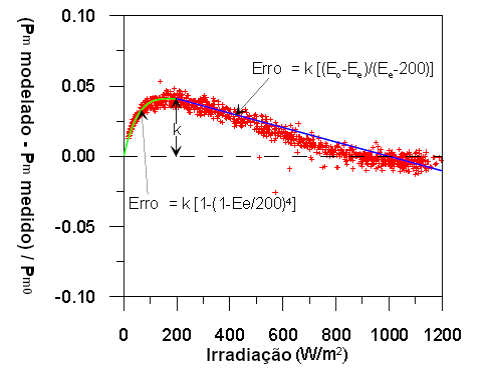
\includegraphics[width=0.725\textwidth]{./Figuras/PVWatts_erro.png}
    \caption{Erro normalizado para um módulo PV de Si multi-cristal.}{Fonte: \cite{Marion}}
   \label{fig:PVWatts_erro}
\end{figure}

Para a correção é utilizado um fator de correção de irradiância, k, que é determinado com a Equação:

\begin{equation}
    k = \frac{P_{pm}(E_L,T) - P_{mmd}(E_L,T)}{P_{m0}}
    \label{eq:ke}
\end{equation}

Onde:

\begin{itemize}
  \item $E_L$ é um valor baixo $\approx 200$ W/m² de irradiância solar.
  
  \item $T$ é um valor da temperatura ambiente quando $ E_L \approx 200$ W/m².

  \item $P_{pm}(E_L,T)$ é o valor calculado pela Equação \ref{eq:pmp} para $E_L$ e $T$.
  
  \item $P_{md}(E_L,T)$ é o valor medido para as condições de $E_L$ e $T$.
\end{itemize}

Assim, as equações finais do modelo ficam:
\newline

Para irradiância $POA > 200$ W/m²:

\begin{equation}
    P_{pm} = P_{m0} [ \frac{POA}{E_0} [1 + \gamma(T_c - T_r)] - k \cdot \frac{E_0 - POA}{E_0 - 200}]
    \label{eq:pmp3}
\end{equation}

Para irradiância $POA < 200$ W/m²:

\begin{equation}
    P_{pm} = P_{m0} [ \frac{POA}{E_0} [1 + \gamma(T_c - T_r)] - k \cdot [1 - (1 - \frac{POA}{200})^4]]
    \label{eq:pmp4}
\end{equation}

\subsection{Conversão CC-CA}

O modelo proposto utiliza uma simples conversão baseada na eficiência do inversor, ou seja, se o conversor tiver 95\% de eficiência a potência CA será:

\begin{equation}
    P_{CA} = P_{mp} \times 0,95
    \label{eq:pca}
\end{equation}

\subsection{Perdas do sistema}

As perdas no sistema que não são explicitamente modeladas, serão fornecidas para o usuário como uma variável de porcentagem de perda de energia gerada.

As perdas representadas por este número incluem os impactos de sujeira, sombreamento, cobertura de neve, incompatibilidade, fiação, conexões, degradação induzida pela luz, classificação da placa de identificação, idade do sistema e disponibilidade operacional \cite{PVWatts}.

Os valores padrão estão listados na Tabela \ref{perdas}:

\begin{table}[htbp]
    \caption{Perdas do sistema \cite{PVWatts}}
        \begin{center}
            \begin{tabular}{ >{\centering\arraybackslash} m{8cm} >{\centering\arraybackslash} m{5cm}  }
                \hline
                Mecanismo de perda & Valor \\ \hline
                Sujeira & 2 \% \\
                Sombreamento & 3 \% \\
                Neve & 0 \% \\
                Incompatibilidade & 2 \% \\
                Fiação & 2 \% \\
                Conexões & 0,5 \% \\
                Degradação induzida por luz & 1,5 \% \\
                Classificação de potência do sistema & 1 \% \\
                Idade & 0 \% \\
                Disponibilidade de operação & 3 \% \\ \hline
                Total & 14 \% (pela Eq. \ref{eq:perdas}) \\
            \end{tabular}
        \end{center}
    \label{perdas}
\end{table}

É importante observar que a perda total não é a soma das perdas individuais. A perda total é calculada multiplicando a redução devido a cada perda $P_i$ (\%) conforme mostrado na Eq.  \ref{eq:perdas}. Assim a perda total padrão do sistema é calculada em 14\% \cite{PVWatts}.

\begin{equation}
    P_{total} (\%) = 100 [1 - \prod_i(1 - \frac{P_i}{100})]
    \label{eq:perdas}
\end{equation}

\newpage
\section{Estruturas para painéis fotovoltaicos}\label{estrutura}

Existe uma série de opções para estrutura de suporte para sistemas PV, podemos ter suportes para telhados, coberturas de garagens, postes, entre outros como até suportes flutuantes para um lago por exemplo. O foco deste estudo é em estruturas que podem ser usadas em telhados, garagens ou estruturas afins.

\begin{figure}[H]
    \centering
    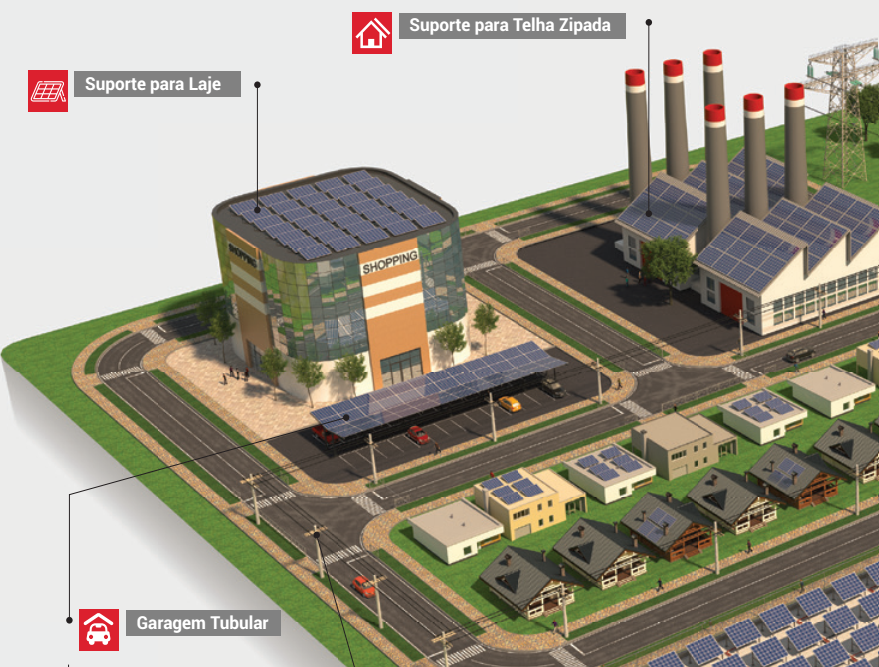
\includegraphics[width=0.95\textwidth]{./Figuras/estruturas.png}
    \caption{Estruturas para painéis fotovoltaicos.}{Fonte: \cite{romagnole}}
   \label{fig:estruturas}
\end{figure}

\subsection{Dados técnicos e custos das estruturas par telhado e garagens}

Nem todas as empresas publicam os custos de seus produtos, mas foi feita uma pesquisa no mês de abril de 2021 e foram encontrados valores e dados técnicos de algumas estruturas o que é suficiente para determinar medidas e custos.

\begin{figure}[H]
    \centering
    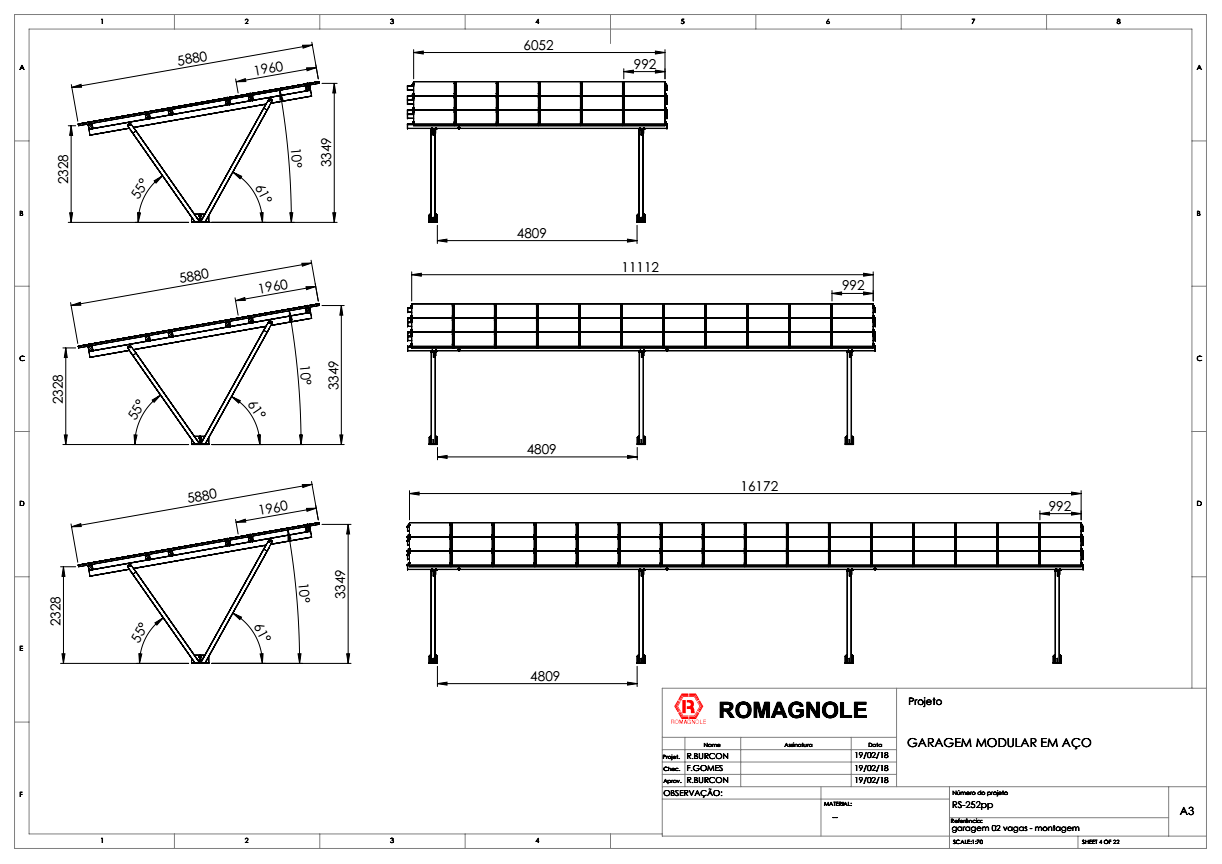
\includegraphics[width=0.8\textwidth]{./Figuras/romagnole_estrutura.png}
    \caption{Garagem modular 2 vagas.}{Fonte: \cite{romagnole_garagem}}
   \label{fig:romagnole_estrutura}
\end{figure}

Na Figura \ref{fig:romagnole_estrutura} são mostradas as medidas da garagem modular Romagnole \textsuperscript{\textregistered} cada divisão cabe dois veículos, na montagem simples, para duas vagas, tem uma área de cobertura de 35,5 m² e na montagem entendida, para 6 vagas, essa área é de 95 m² o custo pode variar de R\$ 5 a 15 mil por vaga sem os painéis PV.

\begin{figure}[H]
    \centering
    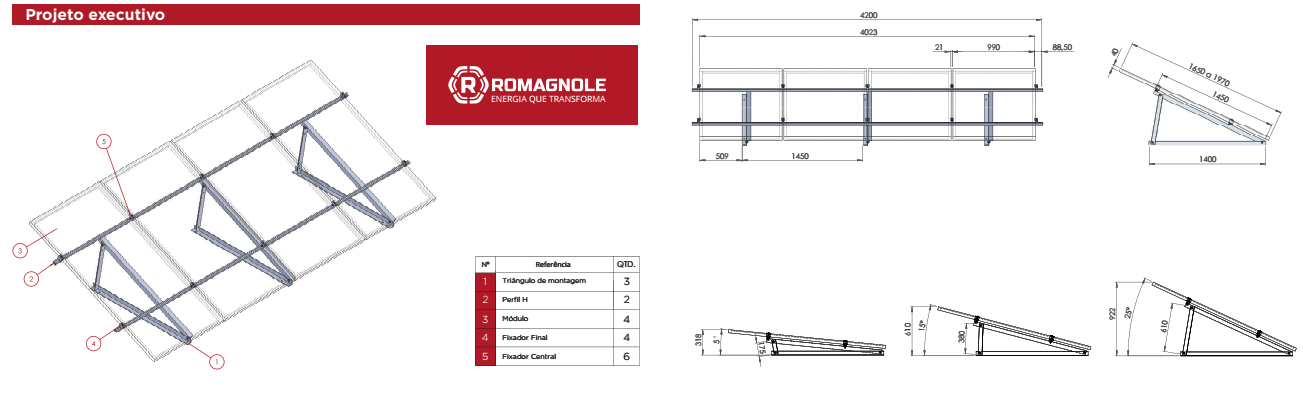
\includegraphics[width=0.95\textwidth]{./Figuras/laje_estrutura.png}
    \caption{Suporte para Laje de Concreto e Telha Angular.}{Fonte: \cite{romagnole_laje}}
   \label{fig:laje_estrutura}
\end{figure}

Na Figura \ref{fig:laje_estrutura}, são mostradas as medidas do suporte para Laje de Concreto e Telha Angular Romagnole\textsuperscript{\textregistered}, este suporte tem encaixe para até 4 painéis com medidas de 1 x 2m com uma área de cobertura de 8,27 m², seu custo pode variar de R\$ 150 a 500 por encaixe de painel, ou seja, o suporte para 4 painéis pode custar até R\$ 2000.

\begin{figure}[H]
    \centering
    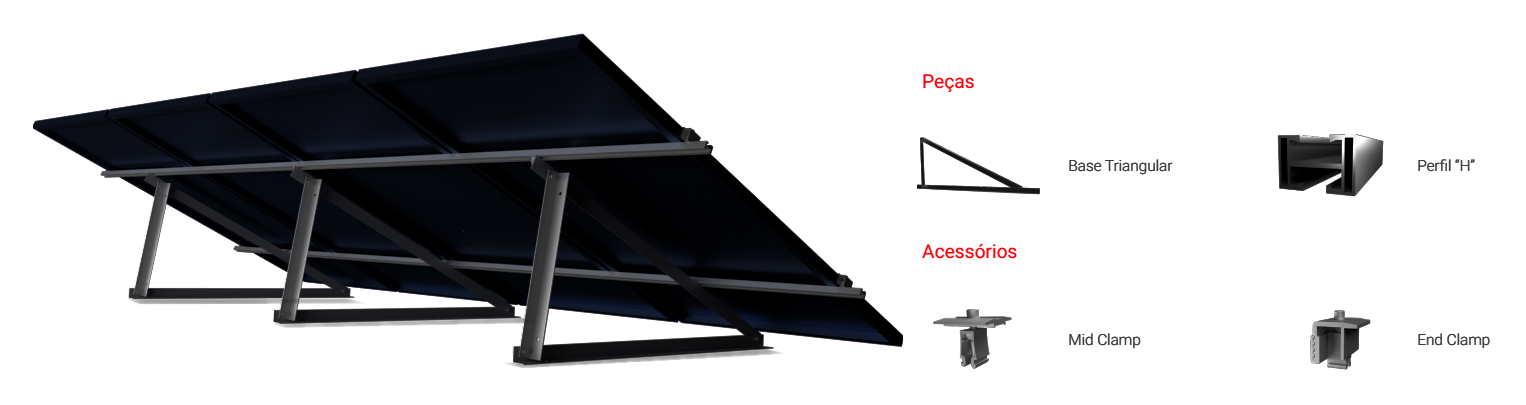
\includegraphics[width=0.85\textwidth]{./Figuras/suporte_laje.png}
    \caption{Suporte para lajes.}{Fonte: \cite{romagnole}}
   \label{fig:suporte_laje}
\end{figure}

A Figura \ref{fig:suporte_laje} mostra os detalhes das peças do kit de suporte para telhas de cerâmica Romagnole\textsuperscript{\textregistered}, este suporte é geralmente feito sob medida, pois as peças dos perfis ``H'', que suportam os painéis, são cortadas a pedido do cliente. Em relação à quantidade de módulos necessária, independente do modelo de telha, os kits tem um custo muito parecido, que pode variar de R\$ 50 a 320, por encaixe de painel, ou seja o suporte para 4 painéis pode custar até R\$ 1280.

Os sites para a pesquisa de custo foram os mesmos da Tabela \ref{preco_pv}.

\subsection{Utilização dos módulos PV nas estruturas}

Em estacionamento, quando já há uma estrutura adequada, utilizada como cobertura, os módulos PV podem ser instalados sobre essa cobertura. De outra forma, o próprio módulos PV pode ser usado como cobertura, como pode ser visualizado na Figura \ref{fig:telhado_pv} .

\begin{figure}[H]
    \centering
    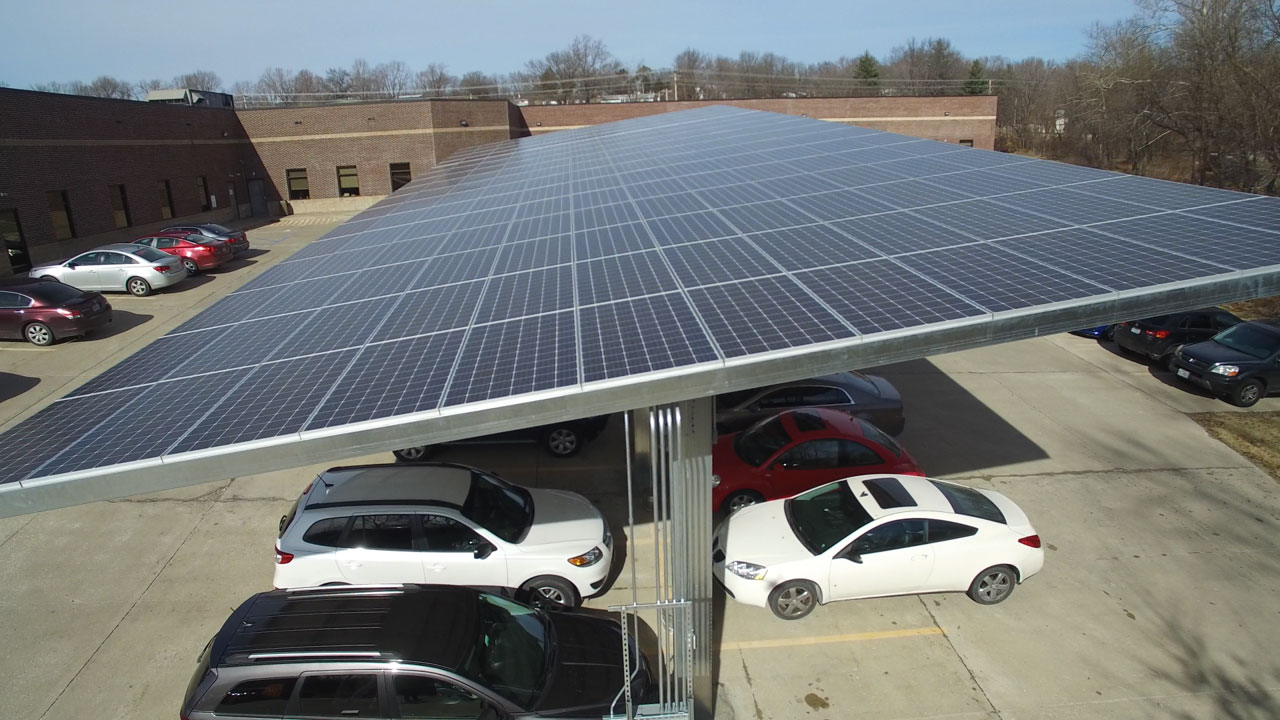
\includegraphics[width=0.85\textwidth]{./Figuras/telhado_pv.jpg}
    \caption{Módulos PV usados como cobertura.}{Fonte: \cite{soliens}}
   \label{fig:telhado_pv}
\end{figure}

A utilização de painéis PV não se dá apenas em estruturas rígidas, a empresa pvilion\textsuperscript{\textregistered} vem há anos desenvolvendo o que ela chama de tecido solar de alta resistência conforme pode ser visto na Figura \ref{fig:tecido_solar}, que é um tecido em PVC com células PV flexíveis de filme fino (polímero orgânico), o tecido tem ``bolsas'' que permitem a inserção de painéis, o que torna o material prático pois um módulo PV pode ser substituído facilmente sem que isso afete a cobertura.

\begin{figure}[H]
    \centering
    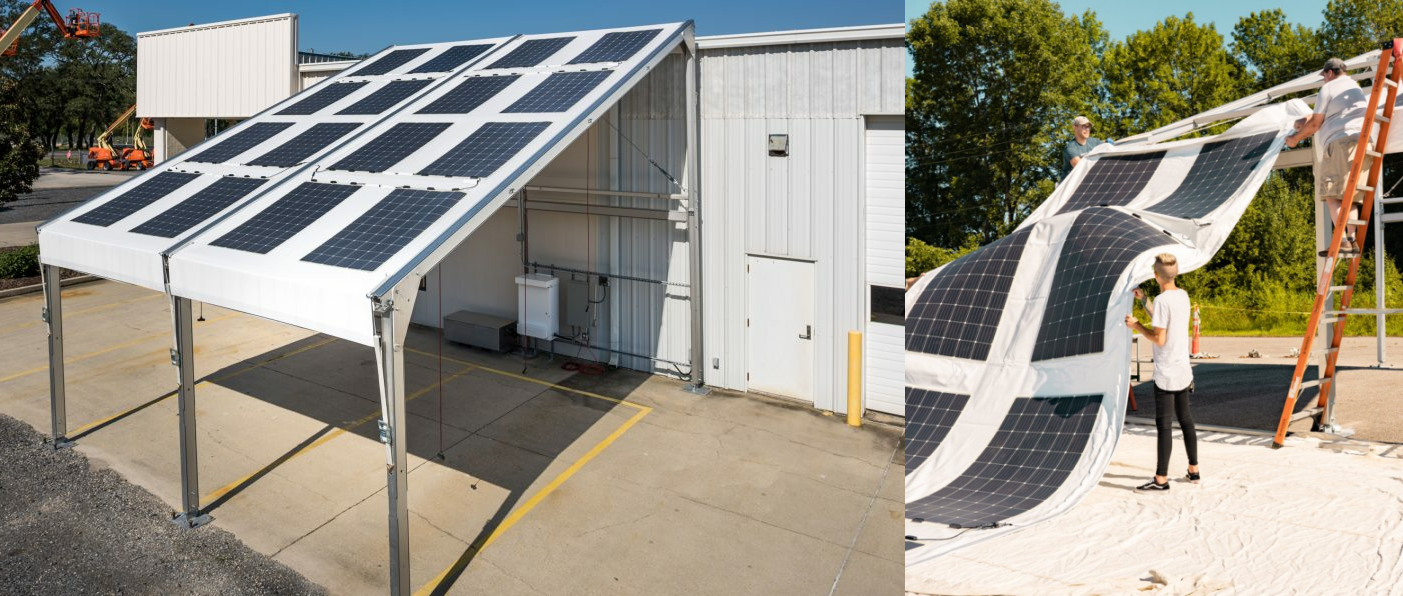
\includegraphics[width=0.9\textwidth]{./Figuras/tecido_solar.png}
    \caption{Tecido solar.}{Fonte: \cite{pvilion}}
   \label{fig:tecido_solar}
\end{figure}

Uma outra opção, é a utilização de telhas ``2 em 1'', conforme se pode visualizar na Figura \ref{fig:telha_pv}, chamada de telha geradora de energia, é um produto nacional, desenvolvido em material com alta resistência química e mecânica, com painéis fotovoltaicos, com células monocristalinas de alta eficiência, totalmente laminadas e seladas, que proporciona isolante térmico, acústico e elétrico. A vantagem deste material é que ele substitui as telhas comuns de uma melhor maneira quando comparado ao utilizar um painel PV como cobertura, pois o painel não foi desenvolvido para ser usado como telhado mas esta telha sim. Em telhados novos, ao invés de montar os painéis sobre telhas, este produto substitui ambos o que proporciona uma economia de até 30\% comparado a outros sistemas \cite{ecotelhasolar}.

\begin{figure}[H]
    \centering
    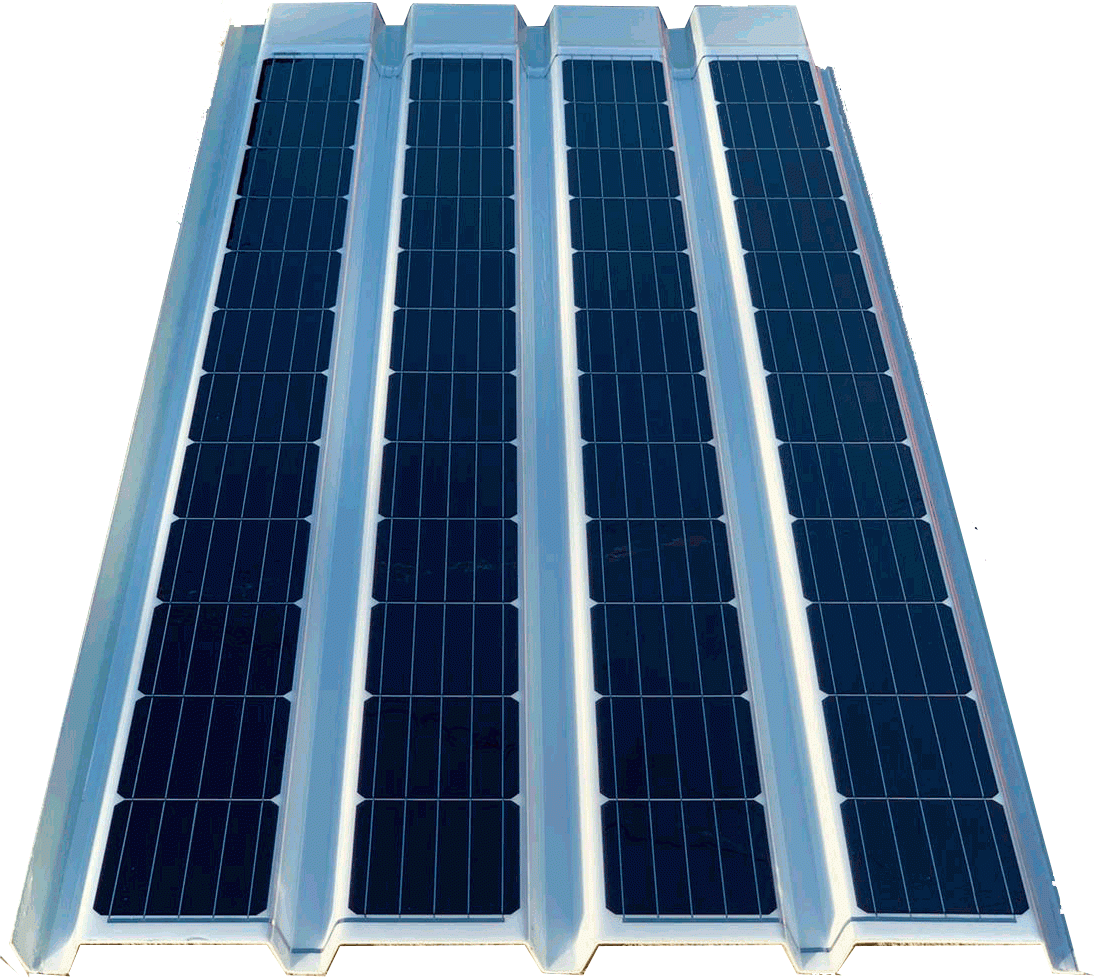
\includegraphics[width=0.6\textwidth]{./Figuras/telha_pv.png}
    \caption{Telhas geradoras de energia.}{Fonte: \cite{ecotelhasolar}}
   \label{fig:telha_pv}
\end{figure}

%https://www.eternit.com.br/dica-da-coruja/telha-fotovoltaica-eternit-solar-o-futuro-e-agora/
%https://super.abril.com.br/tecnologia/telha-que-gera-energia-solar-e-aprovada-no-brasil/

\section{Veículos elétricos}\label{ev}

O objetivo deste trabalho é avaliar apenas veículos 100\% elétricos, ou seja, que utilizam apenas motores elétricos como meio de propulsão. Em comparação a um veículo que usa motor a combustão, um veículo elétrico é muito mais simples. A Figura \ref{fig:ev_partes} ilustra os principais componentes desses veículos.

\begin{figure}[H]
    \centering
    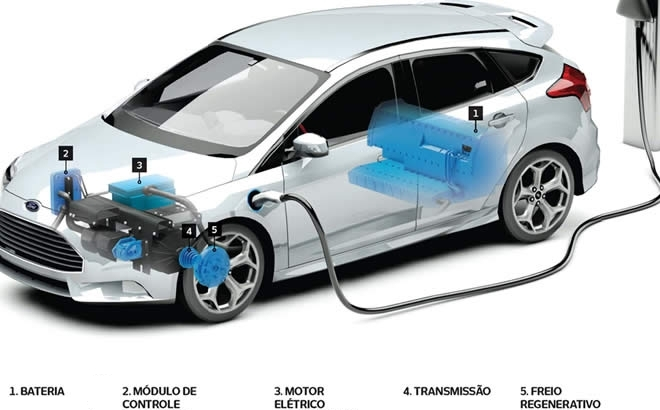
\includegraphics[width=0.75\textwidth]{./Figuras/ev_partes.jpg}
    \caption{O veículo elétrico.}{Fonte: \cite{industriahoje}}
   \label{fig:ev_partes}
\end{figure}

\subsection{Veículos elétricos vendidos no Brasil}

A Tabela \ref{ev_dados} descreve os principais dados usados neste estudo sobre os veículos mais vendidos no Brasil em 2020. Os valores da tabela foram obtidos através dos sites dos fabricantes, o valor de autonomia não demonstra situação de uso real, os fabricantes usam o padrões de teste WLTP ou NEDC que simulam uso real, a diferença na autonomia real pode ser de -25\%.

\begin{table}[htbp]
    \caption{Tabela dados dos veículos mais vendidos Brasil 2020}
        \begin{center}
            \begin{tabular}{ >{\centering\arraybackslash} m{5cm} >{\centering\arraybackslash} m{3.1cm} >{\centering\arraybackslash} m{2cm} >{\centering\arraybackslash} m{3cm} }
                \hline
                Modelo (Montadora) & Bateria & Autonomia & Velocidade de Recarga 80 \% \\ \hline %Primeira e ultima linha adiciona \hline apos \\
                E-TRON \cite{E-TRON} &  95 kWh 396 V & 436 km & 30 m 150 kW \\
                BOLT \cite{BOLT} & 60 kWh 120 V & 416 km & 1 h 55 kW \\
                LEAF  \cite{LEAF} & 40 kWh 350 V & 389 km & 40 minutos 40 kW \\
                I-PACE \cite{I-PACE} & 90,2 kWh 389 V & 470 km & 45 minutos 100 kW \\
                i3  \cite{i3} & 42,2 kWh 352 V & 130 km & 35 minutos 50 kW \\
                KANGOO \cite{KANGOO} & 24 kWh 400 V & 200 km & 6 horas 22 kW \\
                IEV 40 \cite{IEV40} & 40 kWh 400 V & 300 km & 8 horas 6,6 kW \\
                ZOE \cite{ZOE} & 41 kWh 400 V & 317 km & 50 minutos 50 kW \\
                IEV 20 \cite{IEV20} & 41 kWh 326 V & 400 km & 8 horas 6,6 kW \\
                EQC \cite{EQC} & 80 kWh 405 V & 421 km & 35 minutos 100 kW \\ \hline
            \end{tabular}
        \end{center}
    \label{ev_dados}
\end{table}

A Figura \ref{fig:Audi-e-tron-charging-session} demonstra a potência, em kW, que o veículo Audi E-TRON consegue carregar em relação à carga da bateria, para manter a vida útil das baterias dos veículos. A medida em que a carga da bateria se aproxima de seu valor máximo, a potência da carga diminui, por isso é feita essa estimativa de velocidade de recarga de até 80\%, pois esse é o valor ótimo de carga para a maioria dos veículos. Todos os veículos elétricos (VE) modernos utilizam baterias de íon-lítio, este tipo de bateria é geralmente carregado em dois estágios: na situação de baixa carga, a bateria é carregada usando corrente constante até que a tensão atinja um valor específico, após, passa para o modo de carga com tensão constante. Há outros fatores que também afetam o carregamento das baterias, como a temperatura, por exemplo. 

\begin{figure}[H]
    \centering
    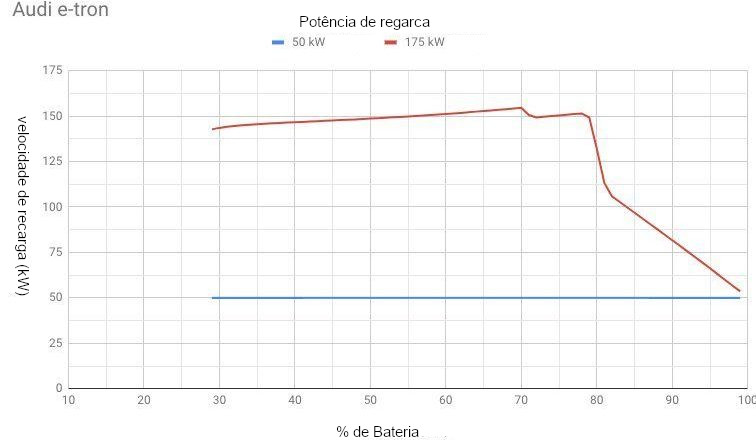
\includegraphics[width=0.775\textwidth]{./Figuras/Audi-e-tron-charging-session.jpg}
    \caption{Audi E-TRON, carregamento de 29 a 100 \% em uma estação de 150 kW de potência VS 50 kW.}{Fonte: \cite{electrek}}
   \label{fig:Audi-e-tron-charging-session}
\end{figure}

As baterias de íon-lítio não podem ser carregadas quando sua temperatura está muito baixa (5°C ou menos), o mesmo ocorre quando a temperatura sobe para mais de 50°C, por isso a maioria dos VE é equipado com um sistema de regulagem de temperatura da bateria, muito similar com o sistema usado para regular a temperatura do motor de veículos à combustão. Na Figura \ref{fig:tesla_cooling} é mostrado o diagrama do sistema de resfriamento da bateria do Tesla Modelo 3.

\begin{figure}[H]
    \centering
    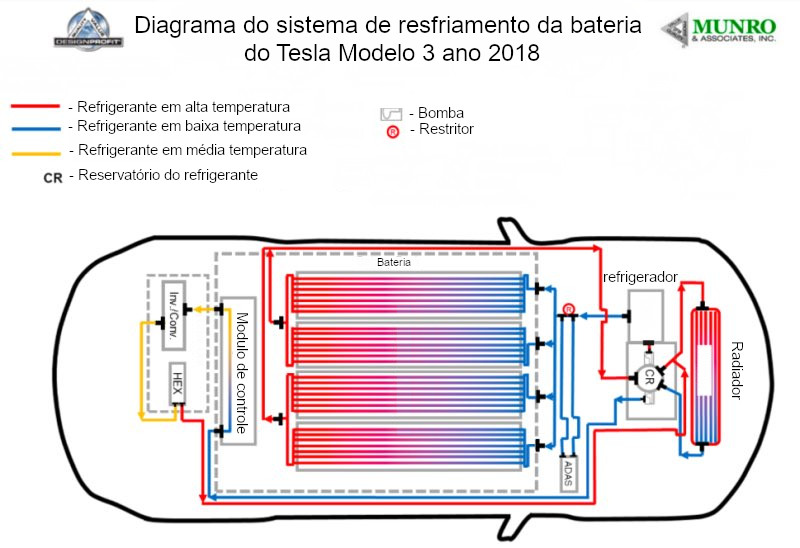
\includegraphics[width=0.75\textwidth]{./Figuras/tesla_cooling.jpg}
    \caption{Diagrama do sistema de resfriamento da bateria do Tesla Modelo 3.}{Fonte: \cite{leandesign}}
   \label{fig:tesla_cooling}
\end{figure}

\subsection{O custo dos veículos elétricos no Brasil}

A Tabela \ref{ev_custo} demonstra o preço e a quantidade dos veículos mais vendidos no Brasil em 2020, levantamento feito pelo site \cite{Motorshow} em relação à lista de veículos comercializados em 2020.

\begin{table}[htbp]
    \caption{Tabela preço dos veículos mais vendidos Brasil 2020 \cite{Motorshow}}
        \begin{center}
            \begin{tabular}{ >{\centering\arraybackslash} m{2cm}
            >{\centering\arraybackslash} m{2cm}
            >{\centering\arraybackslash} m{7cm}  >{\centering\arraybackslash} m{2cm}}
                \hline
                Posição & Unidades vendidas & Modelo (Montadora) & Preço (R\$) \\ \hline %Primeira e ultima linha adiciona \hline apos \\
                1 & 133 & E-TRON \cite{E-TRON} & 531.990  \\
                2 & 108 & BOLT \cite{BOLT} & 260.790 \\
                3 & 105 & LEAF \cite{LEAF} & 220.000 \\
                4 & 98 & I-PACE \cite{I-PACE} & 508.950 \\
                5 & 81 & i3 \cite{i3} & 253.950 \\
                6 & 65 & KANGOO \cite{KANGOO} & 128.990 \\
                7 & 63 & IEV 40 \cite{IEV40} & 189.900 \\
                8 & 33 & ZOE \cite{ZOE} & 203.678 \\
                9 & 29 & IEV 20 \cite{IEV20} & 139.900 \\
                10 & 27 & EQC \cite{EQC} & 575.000 \\ \hline
            \end{tabular}
        \end{center}
    \label{ev_custo}
\end{table}

Não existe modelo de fabricação nacional, assim todos os veículos são importados e a maioria dos veículos elétricos produzidos hoje é produzida para o mercado de carros mais luxuosos. Como o preço dos veículos está vinculado ao Dólar americano, cuja cotação nos últimos anos aumentou muito, fazendo com que o preço de um veículo seja muito alto para o mercado nacional. O valor deses veículos poderia ser ainda maior no Brasil, mas como há isenção de imposto de importação, tem-se algum incentivo, no entanto, é cobrado o Imposto sobre Produtos Industrializados (IPI) que apresenta uma alíquota de 9\%.

\subsection{Autonomia dos veículos elétricos} \label{media_ev}

A Tabela \ref{ev_gas} demonstra um simples comparativo sobre a diferença de preços entre veículos elétricos e veículos à gasolina. A autonomia de veículos elétricos ainda é o ponto mais fraco, porém a eficiência é o mais forte. Na Tabela \ref{ev_gas} foi usado o valor médio de consumo em relação aos veículos da Tabela \ref{ev_dados}, que é 133 Wh/Km. O custo do kWh é a média do custo cobrado pelas distribuidoras. De a cordo com ANEEL \cite{ANEEL_TARIFA} R\$ 0,8675 kWh (R\$ 0,5783 kWh antes da tributação). A distância de 15 Km é a média de consumo por litro de gasolina dos veículos mais vendidos no Brasil \cite{uol_veiculos_consumo}, o custo do combustível segundo \cite{agenciabrasil} em novembro 2021, foi de R\$ 7 por litro, assim é possível concluir que o custo por Km de um veículo elétrico é quase seis vezes menor, e este é um valor baixo, quando comparado com outras regiões do mundo onde o custo da energia elétrica é menor e que não estamos utilizando aqui a autonomia do veículo elétrico mais eficiente possível.

\begin{table}[htbp]
    \caption{Comparativo autonomia veículos elétrico e gasolina}
        \begin{center}
            \begin{tabular}{ >{\centering\arraybackslash} m{3cm} >{\centering\arraybackslash} m{4cm} >{\centering\arraybackslash} m{4cm}  }
                \hline
                Tipo & Distância &  Custo \\ \hline %Primeira e ultima linha adiciona \hline apos \\
                Elétrico & 15 Km & R\$  1,735 (2 kWh) \\
                Gasolina & 15 Km & R\$ 7 (1 Litro)\\ \hline
            \end{tabular}
        \end{center}
    \label{ev_gas}
\end{table}

\section{Estação de recarga para veículos elétricos}

Veículos elétricos armazenam sua energia em baterias. A medida que a energia é usada se torna necessário recarregar as baterias. Para isso, os veículos devem ser conectados a estações de recarga. Estas estações podem ser classificadas, quanto a velocidade de recarga, da seguinte forma:

\begin{itemize}
  \item \textbf{Carregadores ultrarrápidos (Rapid chargers)} com potência de recarga de 40 até 350 kW;
  
  \item \textbf{Carregadores rápidos (Fast Chargers)} com potência de recarga de 7 até 22 kW;
  
  \item \textbf{Carregadores lentos (Slow chargers)} com potência de recarga de 3 até 6 kW.
\end{itemize}

O grande problema das estações de recarga é a compatibilidade da estação com o veículo, tanto na questão da potência de carga quanto no tipo de conector usado. A indústria automobilística não estabeleceu padrão internacional para o sistema, nos seguintes subtópicos isto é relatado com mais detalhes juntamente com as diferenças entre os tipos de estações.

\subsection{Carregadores ultrarrápidos (Rapid chargers)}

Os carregadores ultrarrápidos são os modelos mais rápidos para carregar um VE, porém, nem todos os veículos podem usá-lo. Quando é possível (dependendo do veículo) a recarga de até 80\% ocorre em 20 minutos. Este tipo de estação se encontra em locais públicos ou privados destinados à recarga de vários veículos.

\begin{figure}[H]
    \centering
    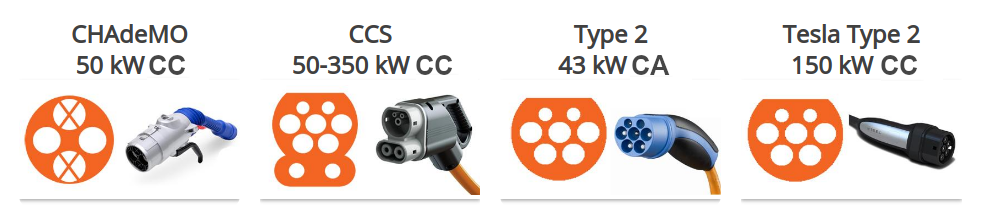
\includegraphics[width=0.8\textwidth]{./Figuras/rapid_chargers.png}
    \caption{Tipos de conectores usados em carregadores ultrarrápidos.}{Fonte: \cite{ev_conect_zap}}
   \label{fig:rapid_chargers}
\end{figure}

A figura \ref{fig:rapid_chargers} mostra os diferentes modelos de conectores encontrados no mundo para este tipo de estação, carregadores de até 43 kW entregam tensão CA ao veículos, porém, todos os de 50kW ou mais entregam tensão CC. Essas estações CC convertem a tensão CA da rede para CC, que por sua vez, é entregue diretamente à bateria do veículo, assim ignorando o conversor CA-CC do veículo, este processo diminui o custo e tamanho do inversor do veículo mas permite que este veículo carregue tanto com CA quando com CC. Os modelos EV que usam o carregamento rápido CHAdeMO incluem o Nissan Leaf e o Mitsubishi Outlander PHEV. Os modelos compatíveis com CCS incluem BMW i3, Kia e-Niro e Jaguar I-PACE. O Modelo 3, o Modelo S e o Modelo X da Tesla são exclusivamente capazes de usar a rede Supercharger, enquanto o único modelo capaz de fazer uso máximo do carregamento rápido CA é o Renault Zoe \cite{ev_conect_zap}.

\begin{figure}[H]
    \centering
    \includegraphics[width=0.4\textwidth]{./Figuras/estacao_ultra_rapida.png}
    \caption{Estação de recarga ultrarrápidos WEG WEMOB Station.}{Fonte: \cite{weg_estacao}}
   \label{fig:estacao_ultra_rapida}
\end{figure}

Na Figura \ref{fig:estacao_ultra_rapida} é mostrada a estação de recarga ultrarrápidos WEG WEMOB Station. Essa estação tem capacidade de recarga rápida e ultra rápida de até 150 kW, e é alimentada com tensão trifásica 380V, disponível com até três modelos de carregadores CHAdeMO, CCS e Tipo 2. Ela apresenta um custo entre 40 mil reais e 100 mil reais \cite{weg_estacao}.

\subsection{Carregadores rápidos (Fast chargers)}

Os carregadores rápidos são os modelos mais comumente encontrados para carregar um VE, quase todos veículos podem usá-lo, em carregadores com potência de até 7 kW, o tempo de recarga de até 80\% ocorre de 4 a 6 horas, em carregadores de 22 kW 1 a 2 horas. Este tipo de estação se encontra em locais públicos ou privados destinados à recarga de vários veículos.

\begin{figure}[H]
    \centering
    \includegraphics[width=0.7\textwidth]{./Figuras/fast_chargers.png}
    \caption{Tipos de conectores usados em carregadores rápidos.}{Fonte: \cite{ev_conect_zap}}
   \label{fig:fast_chargers}
\end{figure}

A Figura \ref{fig:fast_chargers} mostra os diferentes modelos de conector encontrados no mundo para este tipo de estação, todos entregam tensão CA ao veículo com uma potência máxima de 7 até 22 kW. Quase todos os EVs e PHEVs são capazes de carregar em unidades Tipo 2, pelo menos com o cabo correto. É de longe o padrão de ponto de carregamento público mais comum, a maioria dos proprietários de VE terá um cabo com conector Tipo 2 no lado do carregador. O tipo 1 pode ser usado por um Nissan Leaf de primeira geração, mas não por um Leaf de segunda geração, que tem uma entrada Tipo 2 \cite{ev_conect_zap}.

\begin{figure}[H]
    \centering
    \includegraphics[width=0.35\textwidth]{./Figuras/estacao_rapida.png}
    \caption{Estação de recarga rápida WEG WEMOB Parking.}{Fonte: \cite{weg_estacao}}
   \label{fig:estacao_rapida}
\end{figure}

Na Figura \ref{fig:slow_chargers} é mostrada a estação de recarga rápida WEG WEMOB Parking. Essa estação tem capacidade de recarga rápida de até 22 kW, é alimentada com tensão monofásica ou bifásica 127/220V ou trifásica 220/380V, disponível com conector Tipo 2. Ela apresenta um custo entre 27 e 35 mil reais \cite{weg_estacao}.

\subsection{Carregadores lentos (Slow chargers)}

Os carregadores lentos são os modelos comercializados para uso doméstico, para veículos que são carregados, por exemplo, durante a noite em casa. Todos os veículos podem usar esse tipo de carregador, desde que, tenha o cabo adequado, o tempo de recarga de até 80\% entre 6 a 12 horas. Este tipo de estação se encontra em residências ou condomínios, e é destinado à recarga de apenas um veículo.

\begin{figure}[H]
    \centering
    \includegraphics[width=1\textwidth]{./Figuras/slow_chargers.png}
    \caption{Tipos de conectores usados em carregadores lentos.}{Fonte: \cite{ev_conect_zap}}
   \label{fig:slow_chargers}
\end{figure}

A Figura \ref{fig:slow_chargers} mostra os diferentes modelos de conector encontrados no mundo para este tipo de estação, todos entregam tensão CA ao veículo com uma potência máxima de 3 até 6 kW. Todos os EVs podem ser carregados usando pelo menos um dos conectores lentos acima, desde que utilizem o cabo apropriado. A maioria das unidades domésticas tem a mesma entrada Tipo 2 encontrada em carregadores públicos, ou tem um cabo adaptador para Tipo 1. \cite{ev_conect_zap}.

\begin{figure}[H]
    \centering
    \includegraphics[width=0.3\textwidth]{./Figuras/estacao_lenta.png}
    \caption{Estação de recarga lenta WEG WEMOB Wall}{Fonte: \cite{weg_estacao}}
   \label{fig:estacao_lenta}
\end{figure}

A Figura \ref{fig:estacao_lenta} temos a estação de recarga lenta WEG WEMOB Wall. Essa estação tem capacidade de recarga rápida de até 7,4 kW, e é alimentada com tensão monofásica ou bifásica 127/220V, disponível com conector Tipo 2. Ela apresenta um custo entre 7,5 e 10 mil reais \cite{weg_estacao}.

\begin{figure}[H]
    \centering
    \includegraphics[width=0.7\textwidth]{./Figuras/tipe_2_to_1.jpg}
    \caption{Cabo adaptador VE Tipo 2 para Tipo 1.}{Fonte: \cite{EVSE}}
   \label{fig:tipe_2_to_1}
\end{figure}

A Figura \ref{fig:tipe_2_to_1} mostra um cabo para VE adaptador Tipo 2 para Tipo 1. Devido a essa grande variedade de modelos diferentes de conectores, a indústria desenvolveu vários tipos de adaptadores. Alguns veículos já são vendidos com alguns desses adaptadores.

\subsection{Instalação de estação de recarga}

Como qualquer projeto de instalação elétrica, a instalação de uma estação de recarga deve seguir as normas e regulamentações locais, a Enel (antiga Eletropaulo) empresa de distribuição elétrica do estado de São Paulo, disponibiliza em seu site  \cite{Eletropaulo} um documento contendo os critérios para o atendimento de solicitações de ligação nova ou alteração de carga de unidades consumidoras que contenham estações de recarga de veículo elétrico. Os dispositivos regulamentares e normas técnicas deste documento são:

\begin{itemize}
    \item ABNT NBR 5410 – Instalações elétricas de baixa tensão.
    \item ABNT NBR IEC 61851-1 - Sistema de recarga condutiva para veículos elétricos – Parte 1: Requisitos gerais.
    \item ABNT NBR IEC 61851-21 - Sistema de recarga condutiva para veículos elétricos - Parte 21: Requisitos de veículos elétricos para a conexão condutiva a uma alimentação em corrente alternada ou contínua.
    \item ABNT NBR IEC 61851-22 - Sistema de recarga condutiva para veículos elétricos - Parte 22: Estação de recarga em corrente alternada para veículos elétrico.
    \item ABNT NBR IEC 62196-1 - Plugues, tomadas, tomadas móveis para veículo elétrico e plugues fixos de veículos elétricos - recarga condutiva para veículos elétricos - Parte 1: Requisitos gerais.
    \item ABNT NBR IEC 62196-2 - Plugues, tomadas, tomadas móveis para veículo elétrico e plugues fixos de veículo elétrico - recarga condutiva para veículo elétrico - Parte 2: Requisitos dimensionais de compatibilidade e de intercambiabilidade para os acessórios em C.A. com pinos e contatos tubulares.
    \item LIG BT 2014 - Fornecimento de energia elétrica em tensão secundária de distribuição.
    \item LIG MT 2011 - Fornecimento de energia elétrica em tensão primária de distribuição.
    \item Resolução Normativa ANEEL nº 414, de 9 de setembro de 2010.
    \item Resolução Normativa ANEEL nº 819, de 19 de junho de 2018.
\end{itemize}

Estas normas visam garantir que as estações sejam seguras para o uso tanto para as pessoas quanto para seus veículos e em conjunto não causem problemas ou perturbações para a rede elétrica. Dependendo da localidade onde a instalação será feita outras normas ou regras podem ter que ser atendidas.

A Resolução Normativa ANEEL nº 819, de 19 de junho de 2018 \cite{ren2018819} estabelece os procedimentos e as condições para a realização de atividades de recarga de veículos elétricos. Essa resolução estabelece que a distribuidora local de energia deve ser sempre comunicada nos seguintes casos:

\begin{itemize}
    \item[--] Solicitação de fornecimento inicial;
    \item[--] Aumento ou redução de carga; ou
    \item[--] Alteração do nível de tensão.
\end{itemize}

%TRABALHOS RELACIONADOS verificar possibilidade

%\section{Titulo}\label{historia}
%\subsection{subtitulo 1}
%  Explicação das bibliogáfias dos Freios ABS e CBS